% =====================================================================
% Draft-JHEP-Frozen.tex  -- GENERATED, DO NOT EDIT BY HAND
% Generated by scripts/make_frozen_manuscript.py from
%   Draft-JHEP-Active-v6.tex  +  results/jhep_frozen/claim_ledger.csv
% config hash 278e438b94465564
% Every quantitative value below is read from the ledger at generation
% time; none is hard-coded in this file's source of truth.
% =====================================================================
% =====================================================================
% FROZEN SUBMISSION SOURCE - GENERATED, DO NOT EDIT BY HAND
% Frozen-metric checklist -- RESOLVED from the frozen claim ledger
% (results/jhep_frozen/claim_ledger.csv). Status counts per work
% package are shown; every row carries its own estimator class,
% seed set, uncertainty, script, config hash and git commit.
% FM-01 -> WP-0: 1 accepted, 0 failed_gate, 1 ledger rows
% FM-02 -> WP-B: 7 accepted, 1 failed_gate, 8 ledger rows
% FM-03 -> WP-F: 3 accepted, 3 failed_gate, 6 ledger rows
% FM-04 -> WP-C: 12 accepted, 0 failed_gate, 12 ledger rows
% FM-05 -> WP-D: 14 accepted, 0 failed_gate, 14 ledger rows
% FM-06 -> WP-G: 2 accepted, 0 failed_gate, 2 ledger rows
% FM-07 -> WP-B: 7 accepted, 1 failed_gate, 8 ledger rows
% FM-08 -> WP-H: 26 accepted, 0 failed_gate, 26 ledger rows
% FM-09 -> WP-H: 26 accepted, 0 failed_gate, 26 ledger rows
% FM-10 -> WP-A: 113 accepted, 15 failed_gate, 160 ledger rows
% FM-11 -> WP-A: 113 accepted, 15 failed_gate, 160 ledger rows
% FM-12 -> WP-E: 6 accepted, 0 failed_gate, 6 ledger rows
% =====================================================================
\documentclass[a4paper,11pt]{article}
\pdfoutput=1

\usepackage{jheppub}
\usepackage{amsmath,amssymb,mathtools,amsthm}
\usepackage{graphicx}
\usepackage{booktabs}
\usepackage{array,tabularx}
\usepackage{xcolor}
\graphicspath{{figures_jhep_frozen/}}

\newcommand{\E}{\mathbb{E}}
\newcommand{\CN}{\mathcal{N}}
\newcommand{\one}{\mathbf{1}}
\newcommand{\Vir}{\mathrm{Vir}}
% All claim-gate anchors have been resolved from the frozen
% claim ledger; see the checklist above and the ledger table.
\newcommand{\ArchiveDOI}{\texttt{TO-BE-INSERTED}}

\newtheorem{definition}{Definition}[section]
\newtheorem{proposition}[definition]{Proposition}
\newtheorem{theorem}[definition]{Theorem}
\newtheorem{lemma}[definition]{Lemma}
\newtheorem{corollary}[definition]{Corollary}
\newtheorem{remark}[definition]{Remark}

\title{\boldmath Virasoro Symmetry in Neural Network Field Theories}

\author[a]{Brandon Robinson}

\affiliation[a]{Institute of Physics, University of Amsterdam,
904 Science Park, 1098 XH Amsterdam, The Netherlands}

\emailAdd{b.j.robinson@uva.nl}

\abstract{
We construct a random-feature neural realization of the chiral free boson in
which the probabilistic and operator-algebraic structures are kept distinct.
A regulated Log-Kernel layer produces the logarithmic scalar covariance and a
chiral current kernel in a finite scaling window.  In the conformal limit, the difference of the two radial contour orderings
induces the mode pairing $m\delta_{m+n,0}$.  At finite regulators the
pairing is radius dependent, with deviations controlled by current-kernel
non-holomorphy.  Finite-feature architectures are tested before
canonicalization through pairing leakage, raw Sugawara residuals, and Ward
identities.  Canonical quantization of the induced pairing gives the
Heisenberg readout, while truncated Sugawara generators satisfy the Virasoro
algebra exactly as linear maps on low-level filtered Fock subspaces, with
central charge $c=1$.  Darboux normalization is used as a finite-coordinate
correction and not as architecture-selection evidence.  We include charged
sectors and vertex operators, and formulate the corresponding ordered-pairing
construction for the Neveu--Schwarz fermion and the $\mathcal N=1$
super-Virasoro algebra.
}

\begin{document}
\maketitle
\begin{center}
\fbox{\parbox{0.93\textwidth}{\centering
\textbf{FROZEN SUBMISSION SOURCE.} Every quantitative statement in this manuscript is generated from the frozen claim ledger \texttt{results/jhep\_frozen/claim\_ledger.csv} by \texttt{scripts/make\_frozen\_manuscript.py}; none is hard-coded in this source.}}
\end{center}
\flushbottom

% =====================================================================


% CHRONOLOGY / PRIORITY NOTE:
% Do not use later NNFT anomaly or neural string-theory papers as prior
% evidence or independent validation. They appeared after the original draft
% and cite the present work prominently.

\section{Introduction}
\label{sec:introduction}

Infinite-width neural networks with random parameters converge, under broad
conditions, to Gaussian processes whose kernels are determined by the
architecture and parameter prior
\cite{Neal:1996,NIPS1996_ae5e3ce4,Lee:2017wiy}.  This observation underlies
neural-network field theory (NNFT), in which random neural ensembles provide
explicit Euclidean random fields and finite width supplies controlled
non-Gaussian corrections
\cite{Halverson:2020trp,Halverson:2021aot,Dyer:2019uzd,Yaida:2020,
Roberts:2021principles,Demirtas:2023fir,Ferko:2026universality}.  Symmetries may
be engineered through parameter distributions and architecture
\cite{Maiti:2021fpy}.  Conformal neural fields and defect constructions
provide relevant earlier context
\cite{Halverson:2024axc,Capuozzo:2025ozt}.  The present work asks a more
specific two-dimensional question: when does a neural architecture select the
chiral pairing whose quantization carries the Virasoro algebra?

Matching a Euclidean two-point function is not sufficient.  A commuting
random field may reproduce a logarithmic covariance without defining
noncommutative current modes, a Fock representation, normal ordering, a
central extension, or the Ward action of a local stress tensor.  This
distinction is especially sharp in two dimensions, where global conformal
covariance is enlarged to the Virasoro symmetry of the chiral operator algebra
\cite{Belavin:1984vu,DiFrancesco:1997nk,Kac:1998}.  The reconstruction of
operator data from Euclidean correlation functions is itself a nontrivial
problem
\cite{Osterwalder:1973}; we therefore keep the Euclidean neural ensemble and
its quantized readout conceptually separate.

The construction has two architecture-dependent steps followed by an
operator-algebraic step:
\begin{equation}
\begin{aligned}
\text{Log-Kernel features}
&\longrightarrow K_{JJ}^{(N,\Lambda)}
\longrightarrow \omega^{(N,\Lambda)}
\longrightarrow \text{pre-Darboux convergence},
\\
(V,\omega^{(N,\Lambda)})
&\longrightarrow \text{canonical quantization}
\longrightarrow \text{Sugawara readout}
\longrightarrow \mathrm{Vir}.
\end{aligned}
\label{eq:architecture-chain}
\end{equation}
The first line is tested before any coordinate transformation.  The second is
the quantization of the pairing selected by the first.  In particular,
ordinary stochastic covariance is never identified with a commutator.

The classical layer is a regulated random Fourier feature model with
rotationally invariant spectral density $p(k)\propto |k|^{-2}$.  In a physical
window the scalar covariance is logarithmic and its holomorphic derivative has
the current singularity
\begin{equation}
K_{JJ}(z,w)\sim \frac{1}{(z-w)^2}.
\end{equation}
The chiral mode pairing is extracted from the \emph{difference} between the
two nested radial contour orderings.  For the conformal current kernel this
ordered discontinuity is exactly $m\delta_{m+n,0}$.  At finite feature width
and Laurent cutoff, the projected form contains architecture-dependent
leakage.  The emergence claim is that this raw pairing, and the raw Sugawara
algebra built from it, converge to their canonical limits before Darboux
normalization.

Darboux normalization plays a narrower role.  Every finite nondegenerate
antisymmetric form is symplectically equivalent to a canonical form.  Exact
post-Darboux closure therefore verifies the canonicalization, quantization,
and Sugawara implementation, but does not select the Log-Kernel architecture.
Architecture selection is tested through the current kernel, the ordered
pairing, the pre-Darboux leakage and residuals, the compatibility of the
canonicalizing map with the physical involution
$\widehat\alpha_m^\dagger=\widehat\alpha_{-m}$, and finite-network Ward
estimators.

The truncated Sugawara construction is naturally related to finite and
lattice approximations of Virasoro generators
\cite{KooSaleur:1994,MilstedVidal:2017,GransSamuelsson:2021,
OsborneStottmeister:2021}.  Our finite-cutoff theorem is formulated as an
exact identity on a low-level filtered Fock subspace: for fixed mode numbers
and fixed Fock level, the truncated generators agree with the continuum
free-boson generators once the oscillator cutoff is sufficiently large.  The
network contribution lies upstream of this theorem: it provides an explicit,
sampleable finite-feature estimator of the chiral pairing and a controlled
family of finite-width deformations.  The observed leading width dependence
is consistent with the $N^{-1/2}$ Monte Carlo rate expected for random-feature
kernel estimation.

The stress tensor is the abelian Sugawara readout
\cite{Sugawara:1968}.  Charged Fock sectors supply vertex operators with
$h_a=a^2/2$, and current and stress-tensor Ward identities test their local
transformation law.  We apply the same ordered-pairing logic to the Cauchy
fermion kernel and formulate the Neveu--Schwarz $\mathcal N=1$ extension,
using standard superconformal mode conventions
\cite{Friedan:1985ge,Frank:2025zuk}.

The paper is organized as follows.  Section~\ref{sec:lk} defines the commuting
Log-Kernel architecture.  Section~\ref{sec:pairing} derives the ordered chiral
pairing, its finite-feature projection, and the physical constraints on
canonicalization.  Section~\ref{sec:quantized} constructs charged Fock sectors
and proves exact filtered-subspace Virasoro closure.  The numerical and
architecture audits are described in section~\ref{sec:audits}, with technical
kernel, projection, canonicalization, algebra, and control conventions in
appendices~\ref{app:kernel}--\ref{app:controls}.  Section~\ref{sec:ward}
treats primaries and Ward identities, section~\ref{sec:susy} gives the NS
extension, and appendix~\ref{app:finite-width} records finite-width
non-Gaussianity.


\section{The commuting Log-Kernel architecture}
\label{sec:lk}
% =====================================================================

\subsection{Random Fourier features and the regulated kernel}

Let $x=(x^1,x^2)\in\mathbb{R}^2$ and write
$z=x^1+i x^2$.  The finite-width Log-Kernel field is
\begin{equation}
    \phi_N(x;\Theta)
    =
    \frac{\sigma_\phi}{\sqrt{N}}
    \sum_{j=1}^{N}
    \cos(k_j\cdot x+\gamma_j),
    \qquad
    \gamma_j\sim {\rm Unif}[0,2\pi).
    \label{eq:lk-field}
\end{equation}
The momenta are independent draws from the annular density
\begin{equation}
    p_\Lambda(k)
    =
    \frac{1}{\mathcal Z_\Lambda}
    \frac{\one_{\Lambda_{\rm IR}\leq |k|\leq\Lambda_{\rm UV}}}{|k|^2},
    \qquad
    \mathcal Z_\Lambda
    =
    2\pi\log\frac{\Lambda_{\rm UV}}{\Lambda_{\rm IR}}.
    \label{eq:lk-prior}
\end{equation}
A single realization of \eqref{eq:lk-field} is not translation invariant.
Translation and rotation invariance hold for the ensemble covariance,
\begin{align}
    K_\Lambda(x-y)
    &:=
    \E_\Theta[\phi_N(x)\phi_N(y)]
    \nonumber\\
    &=
    \frac{\sigma_\phi^2}{2}
    \int_{\Lambda_{\rm IR}\leq |k|\leq\Lambda_{\rm UV}}
    d^2k\,p_\Lambda(k)\cos(k\cdot(x-y)).
    \label{eq:finite-kernel}
\end{align}
The infinite-width limit makes the field Gaussian, while
\eqref{eq:finite-kernel} is already independent of $N$.

For separations in the physical window
\begin{equation}
    \Lambda_{\rm UV}^{-1}
    \ll |x-y|
    \ll
    \Lambda_{\rm IR}^{-1},
    \label{eq:physical-window}
\end{equation}
the regulated kernel has the form
\begin{equation}
    K_\Lambda(x-y)
    =
    -\kappa\log\!\big(\mu^2|x-y|^2\big)
    +C_\Lambda
    +\delta K_\Lambda(x-y).
    \label{eq:log-kernel}
\end{equation}
Here $C_\Lambda$ is separation independent, $\delta K_\Lambda$ contains
finite-cutoff corrections, and the field normalization is calibrated so that
$\kappa=1$ in the canonical convention used below.  The statement is therefore
a scaling-window statement, not exact scale invariance at finite regulators.

\subsection{The chiral current kernel}

We use
\begin{equation}
    \partial
    =
    \frac12(\partial_{x^1}-i\partial_{x^2}),
    \qquad
    J_N(z;\Theta)
    =
    i\,\partial\phi_N(z;\Theta).
    \label{eq:current-definition}
\end{equation}
With the convention
\begin{equation}
    \E[\phi(z,\bar z)\phi(w,\bar w)]
    =
    -\log|z-w|^2
\end{equation}
in the conformal window, the target holomorphic current kernel is
\begin{equation}
    K_{JJ}(z,w)
    :=
    \E[J(z)J(w)]
    =
    \frac{1}{(z-w)^2}.
    \label{eq:target-current-kernel}
\end{equation}
At finite cutoffs we write
\begin{equation}
    K^\Lambda_{JJ}(z,w)
    =
    \frac{1}{(z-w)^2}
    +
    \delta K^\Lambda_{JJ}(z,w),
    \label{eq:regulated-current-kernel}
\end{equation}
where \eqref{eq:regulated-current-kernel} is understood for separations inside
\eqref{eq:physical-window}.  The regulated kernel is nonsingular below the UV
resolution scale; consequently, contour extractions below are performed at a
mesoscopic contour radius rather than by taking an unregulated
$\epsilon\to0$ limit.

\subsection{Selection within rotationally invariant power laws}

Consider the restricted architecture class
\begin{equation}
    p_\alpha(k)\propto |k|^{-\alpha}
\end{equation}
with rotational invariance and a free-field stress-tensor ansatz
$T\propto:(\partial\phi)^2:$.  The radial derivative covariance has spectral
weight
\begin{equation}
    G_{\partial\phi}(r)
    \propto
    \int_0^\infty dk\,k^{3-\alpha}J_0(kr).
    \label{eq:powerlaw-current}
\end{equation}
Away from regulator scales, dimensional analysis gives
\begin{equation}
    G_{\partial\phi}(r)\sim r^{-(4-\alpha)}.
\end{equation}
A dimension-one chiral current requires a two-point function scaling as
$r^{-2}$.  Within this restricted class, the condition therefore fixes
$\alpha=2$.  This is not a uniqueness statement among arbitrary neural
architectures, anisotropic priors, learned spectra, or non-power-law kernels.

\subsection{What the classical layer does not provide}

For each parameter realization, $\phi_N$ and the projected coefficients built
from it are commuting random variables.  In particular,
\begin{equation}
    [a_m(\Theta),a_n(\Theta)]_{\rm pointwise}=0.
\end{equation}
Their ensemble covariance may approximate a radially ordered contraction, but
it is not a quantum commutator.  The classical layer supplies the feature
geometry and the current kernel from which a chiral pairing can be extracted.
The operator algebra is introduced only after that pairing has been defined.

% =====================================================================

\section{Architecture-induced chiral mode geometry}
\label{sec:pairing}

\subsection{Projected neural modes}

Choose a circle $|z|=R$ lying inside the physical window.  The projected
current coordinates are
\begin{equation}
a_m^{(N)}(R;\Theta)
=
\oint_{|z|=R}\frac{dz}{2\pi i}\,z^m J_N(z;\Theta),
\qquad m\in\mathbb Z.
\label{eq:classical-mode-projection}
\end{equation}
The Jacobi--Anger expansion gives the Bessel-weighted finite feature map
recorded in appendix~\ref{app:mode-projection}.  These coordinates are
commuting random variables.  The nonzero modes are used to extract the chiral
pairing, while the zero mode is adjoined explicitly in
section~\ref{sec:charged-sectors}.

For the finite projection audit we use
\begin{equation}
\mathcal M_\Lambda^\times
=
\{-\Lambda,\ldots,-1,1,\ldots,\Lambda\}.
\label{eq:nonzero-mode-window}
\end{equation}
The full charged Fock construction also contains $\alpha_0$.

\subsection{Two radial orderings}

Let $K_{JJ}(z,w)$ be a chiral current kernel in an annulus contained in the
scaling window, and take $R_{\rm out}>R_{\rm in}>0$.  Define
\begin{align}
\mathcal I^{>}_{mn}[K]
&=
\oint_{|z|=R_{\rm out}}\frac{dz}{2\pi i}\,z^m
\oint_{|w|=R_{\rm in}}\frac{dw}{2\pi i}\,w^n K(z,w),
\label{eq:pairing-order-greater}
\\
\mathcal I^{<}_{mn}[K]
&=
\oint_{|z|=R_{\rm in}}\frac{dz}{2\pi i}\,z^m
\oint_{|w|=R_{\rm out}}\frac{dw}{2\pi i}\,w^n K(z,w).
\label{eq:pairing-order-less}
\end{align}
The induced bilinear form is the ordering discontinuity
\begin{equation}
\omega_{mn}[K]
=
\mathcal I^{>}_{mn}[K]-\mathcal I^{<}_{mn}[K].
\label{eq:ordered-discontinuity-pairing}
\end{equation}
Equation~\eqref{eq:ordered-discontinuity-pairing} extracts an ordered chiral
pairing from the kernel; it is not an ordinary covariance matrix and is not
yet a quantum commutator.

\paragraph{Operational finite-feature definition.}
For a fixed momentum sample $\{k_j\}_{j=1}^{N}$, let
\begin{equation}
K_{JJ}^{(N,\Lambda)}(z,w)
=
\mathbb E_{\gamma}\!\left[
J_N(z;\{k_j,\gamma_j\})J_N(w;\{k_j,\gamma_j\})
\,\middle|\,\{k_j\}
\right]
\label{eq:finite-feature-current-kernel}
\end{equation}
be the phase-averaged empirical current kernel, equivalently obtained by
replacing the regulated spectral measure in the exact kernel by the empirical
measure $N^{-1}\sum_j\delta_{k_j}$.  The pairing used in the frozen
architecture audit is operationally
\begin{equation}
\omega_{mn}^{(N,\Lambda)}(R_{\rm in},R_{\rm out})
=
\mathcal I^{>}_{mn}[K_{JJ}^{(N,\Lambda)}]
-
\mathcal I^{<}_{mn}[K_{JJ}^{(N,\Lambda)}].
\label{eq:operational-finite-pairing}
\end{equation}
For each regulator row, choose a strict evaluation interval
$[r_{\min},r_{\max}]$ inside the physical window and write
\begin{equation}
R_0=\sqrt{r_{\min}r_{\max}},\qquad
R_{\rm in}=\frac{R_0}{\sqrt\rho},\qquad
R_{\rm out}=R_0\sqrt\rho .
\label{eq:operational-radii}
\end{equation}
The reference extraction uses $\rho=2$; the radius-stability audit varies both
$R_0$ and $\rho$ while maintaining
$r_{\min}<R_{\rm in}<R_{\rm out}<r_{\max}$.  Every output row records
$R_{\rm in}$, $R_{\rm out}$, $R_0$, and $\rho$:
% RESOLVED FM-10: see the frozen claim ledger (results/jhep_frozen/claim_ledger.csv).

The present released column named
\texttt{radial\_ordered\_projection\_leakage} was produced from the
single-radius Laurent projection matrix $F(R)$ described in
appendix~\ref{app:mode-projection}.  We therefore denote it by
$\epsilon_{\rm leak}^{\rm proj}$ and use it only as a projection-level proxy.
It is not silently identified with the operational two-radius pairing
\eqref{eq:operational-finite-pairing}; the frozen suite recomputes the full
grid with the latter definition.

\begin{proposition}[Current singularity and oscillator pairing]
\label{prop:current-pairing}
For $K_{JJ}(z,w)=(z-w)^{-2}$,
\begin{equation}
\omega_{mn}=m\delta_{m+n,0}.
\label{eq:canonical-pairing}
\end{equation}
\end{proposition}

\begin{proof}
For $|z|>|w|$,
\begin{equation}
\frac{1}{(z-w)^2}
=
\sum_{k\geq0}(k+1)w^k z^{-k-2},
\end{equation}
so the two residues require $k=m-1=-n-1$ and give
\begin{equation}
\mathcal I^{>}_{mn}
=
m\,\mathbf 1_{m>0}\delta_{m+n,0}.
\end{equation}
For $|w|>|z|$,
\begin{equation}
\frac{1}{(z-w)^2}
=
\sum_{k\geq0}(k+1)z^k w^{-k-2},
\end{equation}
which gives
\begin{equation}
\mathcal I^{<}_{mn}
=
(-m)\,\mathbf 1_{m<0}\delta_{m+n,0}.
\end{equation}
Their difference is $m\delta_{m+n,0}$ for every $m\neq0$, and both terms
vanish at $m=0$.
\end{proof}

Proposition~\ref{prop:current-pairing} is the architecture-to-mode step used
throughout the remainder of the paper.

\begin{proposition}[Equivalence with the local residue prescription]
\label{prop:residue-equivalence}
Suppose $K(z,w)$ is meromorphic in the annular region swept when the
$z$-contour is deformed from $R_{\rm out}$ to $R_{\rm in}$, and that its only
intervening singularity is the diagonal $z=w$.  Then
\begin{equation}
\mathcal I^{>}_{mn}[K]-\mathcal I^{<}_{mn}[K]
=
\oint_{|w|=R}\frac{dw}{2\pi i}\,w^n
\oint_{|z-w|=\epsilon}\frac{dz}{2\pi i}\,z^m K(z,w).
\label{eq:residue-ordering-equivalence}
\end{equation}
\end{proposition}

\begin{proof}
Deform the outer $z$-contour through the inner one while keeping the
$w$-contour fixed.  By the residue theorem, the difference between the two
nested contour integrals is the sum of the singularities crossed.  Under the
stated hypothesis this is precisely the small contour around $z=w$.
\end{proof}

Proposition~\ref{prop:residue-equivalence} provides a direct unit test between
the two-ordering implementation and the local-residue audit for a meromorphic
chiral kernel.  At finite spectral cutoff, however, the exact Euclidean
current kernel is not holomorphic and the two prescriptions are not
interchangeable.

\subsection{Finite-cutoff non-holomorphy and radius stability}

Let $\xi=z-w$, $u=\xi\bar\xi$, and write the regulated scalar kernel as
$K_\Lambda(z,w)=k_\Lambda(u)$.  Direct differentiation gives the following
structural statement.

\begin{proposition}[Non-holomorphy of the regulated current kernel]
\label{prop:regulated-nonholomorphy}
The exact regulated current kernel is
\begin{equation}
K_{JJ}^{\Lambda}(z,w)
=
(\bar z-\bar w)^2 k_\Lambda''(u),
\label{eq:radial-current-kernel-form}
\end{equation}
and
\begin{equation}
\partial_{\bar z}K_{JJ}^{\Lambda}(z,w)
=
(\bar z-\bar w)\left[2k_\Lambda''(u)+u k_\Lambda'''(u)\right].
\label{eq:dbar-current-kernel}
\end{equation}
On an interval of $u>0$, the current kernel is holomorphic in $z$ if and only
if
\begin{equation}
k_\Lambda(u)=-A\log u+B u+C
\end{equation}
there.  The affine terms do not contribute to
$K_{JJ}^{\Lambda}$, while $A=1$ gives $(z-w)^{-2}$.
\end{proposition}

\begin{proof}
Equation~\eqref{eq:radial-current-kernel-form} follows from
$-\partial_z\partial_w k_\Lambda(u)$.  Applying $\partial_{\bar z}$ gives
\eqref{eq:dbar-current-kernel}.  Vanishing away from the diagonal is
$u k'''(u)+2k''(u)=0$, whose general solution is
$k(u)=-A\log u+B u+C$.
\end{proof}

Thus the Bessel-regulated kernel is generically non-holomorphic at finite
cutoff.  Consequently, the extracted finite pairing depends genuinely on the
chosen inner and outer radii.  Two complementary bounds quantify this
dependence.

\begin{proposition}[Finite-cutoff pairing error]
\label{prop:finite-pairing-bound}
Let $K_0(z,w)=(z-w)^{-2}$ and
$\delta K=K_{JJ}^{(N,\Lambda)}-K_0$.  On the two contour tori
$T_{oi}=\{|z|=R_{\rm out},|w|=R_{\rm in}\}$ and
$T_{io}=\{|z|=R_{\rm in},|w|=R_{\rm out}\}$,
\begin{align}
\left|\omega_{mn}^{(N,\Lambda)}-m\delta_{m+n,0}\right|
&\le
R_{\rm out}^{m+1}R_{\rm in}^{n+1}
\|\delta K\|_{L^\infty(T_{oi})}
\nonumber\\
&\quad+
R_{\rm in}^{m+1}R_{\rm out}^{n+1}
\|\delta K\|_{L^\infty(T_{io})}.
\label{eq:finite-pairing-bound}
\end{align}
\end{proposition}

\begin{proof}
Subtract the ideal-kernel functionals and bound each normalized contour
integral by its contour length times the supremum norm.  The radii are
positive, so the expression applies to positive and negative integer modes.
\end{proof}

\begin{proposition}[Cauchy--Green radius-variation bound]
\label{prop:radius-variation}
For $R_{\rm out}' > R_{\rm out}>R_{\rm in}$ and a smooth finite-cutoff
kernel,
\begin{align}
&\left|
\mathcal I^>_{mn}(R_{\rm in},R_{\rm out}')
-
\mathcal I^>_{mn}(R_{\rm in},R_{\rm out})
\right|
\nonumber\\
&\qquad\le
\frac{R_{\rm in}^{n+1}}{\pi}
\iint_{A(R_{\rm out},R_{\rm out}')}
|z|^m
\sup_{|w|=R_{\rm in}}
\left|\partial_{\bar z}K_{JJ}^{(N,\Lambda)}(z,w)\right|
\,d^2z .
\label{eq:radius-variation-bound}
\end{align}
Analogous bounds hold when varying the inner contour and for
$\mathcal I^<$, with $z,m$ and $w,n$ exchanged.  The total variation of
$\omega_{mn}^{(N,\Lambda)}$ between two radius pairs is bounded by the sum of
the corresponding four terms.
\end{proposition}

\begin{proof}
Apply the Cauchy--Green formula to $z^mK_{JJ}^{(N,\Lambda)}(z,w)$ on the
annulus between the two outer contours and then take the normalized
$w$-contour integral.  Since $z^m$ is holomorphic on this annulus, only
$\partial_{\bar z}K_{JJ}^{(N,\Lambda)}$ contributes.
\end{proof}

Propositions~\ref{prop:finite-pairing-bound} and
\ref{prop:radius-variation} turn contour dependence into a measurable
regulator diagnostic.  The frozen audit reports
$\omega^{(N,\Lambda)}$ over a grid of $(R_0,\rho)$, the associated
$\bar\partial$ norm from \eqref{eq:dbar-current-kernel}, and a plateau region
in which the pairing is stable:
% RESOLVED FM-11: see the frozen claim ledger (results/jhep_frozen/claim_ledger.csv).

\subsection{Finite-feature pairing and the joint limit}

On $\mathcal M_\Lambda^\times$, write
\begin{equation}
\omega^{(N,\Lambda)}
=
\omega_{\rm can}+\varepsilon^{(N,\Lambda)},
\qquad
(\omega_{\rm can})_{mn}=m\delta_{m+n,0}.
\end{equation}
We use
\begin{align}
\epsilon_{\rm pair}
&=
\frac{\|\omega^{(N,\Lambda)}-\omega_{\rm can}\|_F}
{\|\omega_{\rm can}\|_F},
\\
\epsilon_{\rm leak}
&=
\frac{
\big(\sum_{m+n\neq0}|\omega^{(N,\Lambda)}_{mn}|^2\big)^{1/2}}
{\big(\sum_{m+n=0}|\omega^{(N,\Lambda)}_{mn}|^2\big)^{1/2}}.
\label{eq:pairing-errors}
\end{align}
The architecture-level statement is pre-Darboux convergence:
\begin{equation}
\epsilon_{\rm pair}\longrightarrow0,
\qquad
\epsilon_{\rm leak}\longrightarrow0,
\qquad
\mathcal R_{\rm raw}\longrightarrow0.
\label{eq:predarboux-limit}
\end{equation}
The frozen multi-seed campaign replaces the provisional three-width grid. Fitting $\log Y=c+b\log N+a\log\Lambda$ with regulator fixed effects over ten independent seeds gives the width exponents
\begin{align}
\begin{split}
\epsilon_{\rm samp}\ (\text{sharp annulus}) &: \quad b = -0.494\pm 0.01613, \quad \text{a = 4.527} \\
\epsilon_{\rm pair}\ (\text{sharp annulus}) &: \quad b = -0.456\pm 0.01637, \quad \text{a = 4.489} \\
\epsilon_{\rm leak}\ (\text{sharp annulus}) &: \quad b = -0.037\pm 0.01911, \quad \text{a = 0.1598} \\
\mathcal R_{\rm raw}\ (\text{sharp annulus}) &: \quad b = -0.57\pm 0.01351, \quad \text{a = 3.117} \\
\epsilon_{\rm samp}\ (\text{tapered diagnostic}) &: \quad b = -0.491\pm 0.01573, \quad \text{a = 4.509} \\
\epsilon_{\rm pair}\ (\text{tapered diagnostic}) &: \quad b = -0.491\pm 0.01573, \quad \text{a = 4.508} \\
\epsilon_{\rm leak}\ (\text{tapered diagnostic}) &: \quad b = -0.067\pm 0.01755, \quad \text{a = 0.4754} \\
\mathcal R_{\rm raw}\ (\text{tapered diagnostic}) &: \quad b = -0.539\pm 0.01078, \quad \text{a = 3.408}
\end{split}
\end{align}
The finite-$N$ sampling error about the analytic closed-kernel pairing is statistically indistinguishable from the $N^{-1/2}$ random-feature rate under both regulator classes. Under the sharp annulus of eq.~\eqref{eq:lk-prior} the total pairing error does \emph{not} converge to zero: it saturates on a cutoff-induced floor, and the null $b=-1/2$ is rejected. Under a $15\%$ raised-cosine taper in $\log k$ the same measurement is consistent with $b=-1/2$ and the pairing converges to $m\delta_{m+n,0}$. All rows, exclusions and $p$-values are in \texttt{predarboux\_convergence\_fits.csv}.

\subsection{Darboux canonicalization and the physical involution}

\begin{proposition}[Finite-dimensional Darboux universality]
\label{prop:darboux-universality}
Every nondegenerate real antisymmetric form on a finite even-dimensional
vector space admits an invertible change of basis $S$ such that
\begin{equation}
S\Omega S^T=\Omega_{\rm can}.
\end{equation}
Consequently, post-Darboux Heisenberg and Sugawara closure is not by itself an
architecture-selection test.
\end{proposition}

The physical complex mode space also carries
\begin{equation}
\widehat\alpha_m^\dagger=\widehat\alpha_{-m}.
\label{eq:mode-star}
\end{equation}
Let $C_{mn}=\delta_{m,-n}$.  A complex canonicalizing map is compatible with
\eqref{eq:mode-star} when
\begin{equation}
\overline S\,C=C\,S.
\label{eq:star-compatible-darboux}
\end{equation}
The frozen control campaign therefore records not only symplectic
canonicalization error, but also the defect in
\eqref{eq:star-compatible-darboux} and the positivity of the induced
positive-frequency Fock structure.  Numerical conventions and admissibility
checks are collected in appendix~\ref{app:darboux}.  If a control closes algebraically but
fails these physical conditions, post-Darboux closure becomes a weaker
statement than unitary equivalence of the corresponding readouts.


\section{Quantized readout and the Virasoro algebra}
\label{sec:quantized}

\subsection{Heisenberg quantization}

Given a finite pairing $(V_\Lambda,\omega^{(N,\Lambda)})$, define the
Heisenberg algebra by
\begin{equation}
[\widehat a(v),\widehat a(u)]
=
\omega^{(N,\Lambda)}(v,u)\mathbf 1.
\label{eq:matrix-CCR}
\end{equation}
After a physically admissible canonicalization, the modes obey
\begin{equation}
[\widehat\alpha_m,\widehat\alpha_n]
=
m\delta_{m+n,0}\mathbf 1,
\qquad
\widehat\alpha_m^\dagger=\widehat\alpha_{-m}.
\label{eq:canonical-CCR}
\end{equation}
This is a genuine noncommutative readout.  Its regular irreducible
finite-dimensional phase-space representation is unique up to unitary
equivalence in the sense of the Stone--von Neumann theorem
\cite{Folland:1989}.

\subsection{Charged sectors and zero modes}
\label{sec:charged-sectors}

Adjoin a zero mode and conjugate coordinate,
\begin{equation}
[\widehat q,\widehat\alpha_0]=i,
\qquad
[\widehat\alpha_0,\widehat\alpha_n]=0
\quad(n\neq0).
\end{equation}
For each $a\in\mathbb R$, the charged Fock module $\mathcal F_a$ is generated
from
\begin{equation}
\widehat\alpha_0|a\rangle=a|a\rangle,
\qquad
\widehat\alpha_n|a\rangle=0
\quad(n>0).
\end{equation}
The Sugawara modes are
\begin{equation}
\widehat L_m
=
\frac12\sum_{p\in\mathbb Z}
:\widehat\alpha_{m-p}\widehat\alpha_p:,
\label{eq:full-sugawara}
\end{equation}
and
\begin{equation}
\widehat L_0
=
\frac12\widehat\alpha_0^2+
\sum_{p>0}\widehat\alpha_{-p}\widehat\alpha_p.
\end{equation}
Hence
\begin{equation}
\widehat L_0|a\rangle=\frac{a^2}{2}|a\rangle,
\label{eq:charged-weight}
\end{equation}
which gives $h_a=a^2/2$.  The zero mode changes the representation and primary
weight but not the oscillator central term.

\subsection{Truncated generators and level filtration}

For
\begin{equation}
v=
\widehat\alpha_{-r_1}\cdots\widehat\alpha_{-r_s}|a\rangle,
\qquad r_i>0,
\end{equation}
define the level $\ell(v)=\sum_i r_i$, and let
$\mathcal F_a^{(\le K)}$ be the span of states of level at most $K$.  The
truncated generator is
\begin{equation}
\widehat L_m^{(\Lambda)}
=
\frac12
\sum_{\substack{p\in\mathbb Z\\
|p|\le\Lambda,\ |m-p|\le\Lambda}}
:\widehat\alpha_{m-p}\widehat\alpha_p:.
\label{eq:truncated-sugawara}
\end{equation}
Write
\begin{equation}
m_-=\max(0,-m).
\end{equation}

\begin{lemma}[Support of a Sugawara mode]
\label{lem:sugawara-support}
If $v\in\mathcal F_a^{(\le K)}$ and
\begin{equation}
\Lambda\ge K+m_-,
\label{eq:single-mode-bound}
\end{equation}
then
\begin{equation}
\widehat L_m^{(\Lambda)}v=\widehat L_m v.
\end{equation}
\end{lemma}

\begin{proof}
Consider a normal-ordered summand
$:\widehat\alpha_{m-p}\widehat\alpha_p:$ acting nontrivially on $v$.
If both indices are negative, the summand is pure creation, so $m<0$ and the
total created level is $m_-=|m|$; both indices have magnitude at most $m_-$.
If one index is zero, the other is $m$, and the term is either bounded by
$m_-$ or annihilates a level-$K$ state when $m>K$.  In every remaining
nonzero summand there is a positive annihilation mode of index $s\le K$.
For $m\ge0$, its partner has magnitude at most $K$ whenever the term acts
nontrivially.  For $m<0$, the partner has magnitude at most $K+m_-$.  Thus all
oscillator indices required on $\mathcal F_a^{(\le K)}$ lie inside the
truncation under \eqref{eq:single-mode-bound}.
\end{proof}

\begin{theorem}[Filtered finite-cutoff Virasoro theorem]
\label{thm:filtered-virasoro}
Let $m,n\in\mathbb Z$ and $K\ge0$.  If
\begin{equation}
K+m_-+n_-\le\Lambda,
\label{eq:filtered-bound}
\end{equation}
then, for every $v\in\mathcal F_a^{(\le K)}$,
\begin{equation}
\begin{split}
[\widehat L_m^{(\Lambda)},\widehat L_n^{(\Lambda)}]v
&=
(m-n)\widehat L_{m+n}^{(\Lambda)}v
\\
&\quad+
\frac{1}{12}m(m^2-1)\delta_{m+n,0}\,v.
\end{split}
\label{eq:filtered-virasoro}
\end{equation}
Thus the truncated generators satisfy the $c=1$ Virasoro algebra exactly as
linear maps with domain $\mathcal F_a^{(\le K)}$.
\end{theorem}

\begin{proof}
The mode $\widehat L_n$ maps a level-$\ell$ vector to level $\ell-n$ when the
result is nonzero, and therefore maps
$\mathcal F_a^{(\le K)}$ into
$\mathcal F_a^{(\le K+n_-)}$.  By
lemma~\ref{lem:sugawara-support} and
\eqref{eq:filtered-bound},
\begin{align}
\widehat L_m^{(\Lambda)}
\widehat L_n^{(\Lambda)}v
&=
\widehat L_m\widehat L_n v,
\\
\widehat L_n^{(\Lambda)}
\widehat L_m^{(\Lambda)}v
&=
\widehat L_n\widehat L_m v.
\end{align}
Moreover, $(m+n)_-\le m_-+n_-$, so
$\widehat L_{m+n}^{(\Lambda)}v=\widehat L_{m+n}v$.  Substituting the standard free-boson relation
\cite{DiFrancesco:1997nk,Kac:1998}
\begin{equation}
[\widehat L_m,\widehat L_n]
=
(m-n)\widehat L_{m+n}
+
\frac{1}{12}m(m^2-1)\delta_{m+n,0}\mathbf 1
\end{equation}
proves \eqref{eq:filtered-virasoro}.
\end{proof}

\begin{corollary}[Strong convergence on filtered pieces]
\label{cor:filtered-limit}
For fixed $K,m,n$, equation~\eqref{eq:filtered-virasoro} holds for every
sufficiently large $\Lambda$.  Along the natural inclusions of the filtered
Fock spaces, $\widehat L_m^{(\Lambda)}$ converges strongly on each fixed
filtered piece to $\widehat L_m$.  No operator-norm convergence on the full
Fock space is asserted.
\end{corollary}

The explicit edge remainder outside \eqref{eq:filtered-bound} remains a useful
diagnostic and is described in appendix~\ref{app:formal-audit}; it is no longer
used to define the domain on which the central theorem holds.


\section{Architecture and algebra audits}
\label{sec:audits}

\subsection{Numerical conventions and provenance}

Every final manuscript number is generated by a frozen master suite and
recorded in a claim ledger containing the metric definition, configuration,
seed set, estimator type, uncertainty, source script, output artifact, and git
commit.  The current integration draft uses only quantities reproducible from
the mounted CSV release; entries not present in that release are marked by
% RESOLVED FM-01
(resolved by the frozen claim ledger, whose row count is $235$; see table~\ref{tab:claim-ledger})
analytic closed-kernel identities, deterministic finite-feature calculations,
and sampled finite-network estimators.

The contour and local-residue implementations are required to agree under the
hypotheses of proposition~\ref{prop:residue-equivalence}.  The numerical
canonicalization audit reports ordinary symplectic error, the
$*$-compatibility defect \eqref{eq:star-compatible-darboux}, conditioning, and
positive-frequency vacuum diagnostics.  Full definitions and parameter
tables are collected in appendices~\ref{app:kernel}--\ref{app:controls}.


Table~\ref{tab:provenance-summary} provides the single source-of-truth summary
for the quantitative values retained in this integration draft.
% GENERATED by scripts/make_frozen_manuscript.py
\begin{table}[t]
\centering
\begin{tabular}{@{}lr@{}}
\toprule
Ledger status & Rows \\
\midrule
accepted & 176 \\
diagnostic & 32 \\
failed\_gate & 19 \\
accepted\_with\_caveat & 8 \\
\bottomrule
\end{tabular}
\caption{Single source-of-truth summary of the frozen claim ledger.}
\label{tab:provenance-summary}
\end{table}

% GENERATED by scripts/make_frozen_manuscript.py from claim_ledger.csv
\begin{table}[t]
\centering\footnotesize
\begin{tabular}{@{}llllll@{}}
\toprule
Claim & WP & Value & Uncertainty & Estimator class & Status \\
\midrule
\texttt{wpA\_pairing\_antidiag\_error\_sharp\_annulus\_manuscript} & WP-A & $33$ & $84.55$ & \texttt{deterministic\_finite\_feature} & failed\_gate \\
\texttt{wpA\_nonholomorphy\_sup\_sharp\_annulus\_manuscript} & WP-A & $7.44828\times10^{5}$ & \textsc{unresolved} & \texttt{analytic\_closed\_kernel} & accepted \\
\texttt{wpA\_pairing\_antidiag\_error\_tapered\_log\_window} & WP-A & $12$ & $29.34$ & \texttt{deterministic\_finite\_feature} & accepted \\
\texttt{wpA\_nonholomorphy\_sup\_tapered\_log\_window} & WP-A & $949.155$ & \textsc{unresolved} & \texttt{analytic\_closed\_kernel} & accepted \\
\texttt{wpA\_radius\_plateau\_sharp\_annulus\_manuscript} & WP-A & [0.0470998, 21.2315] & 10 nodes & \texttt{deterministic\_finite\_feature} & accepted \\
\texttt{wpA\_cauchy\_green\_bound\_ratio\_sharp\_annulus\_manuscript} & WP-A & $1.62257\times10^{-5}$ & $1.461\times10^{-4}$ & \texttt{deterministic\_finite\_feature} & accepted \\
\texttt{wpA\_radius\_plateau\_tapered\_log\_window} & WP-A & [0.0470998, 21.2315] & 10 nodes & \texttt{deterministic\_finite\_feature} & accepted \\
\texttt{wpA\_cauchy\_green\_bound\_ratio\_tapered\_log\_window} & WP-A & $0.0173467$ & $1.254$ & \texttt{deterministic\_finite\_feature} & accepted\_with\_caveat \\
\texttt{wpA\_fit\_pairing\_leakage\_sharp\_annulus\_manuscript} & WP-A & $-0.037$ & $0.01911$ & \texttt{deterministic\_finite\_feature} & accepted \\
\texttt{wpA\_fit\_pairing\_relative\_error\_sharp\_annulus\_manuscript} & WP-A & $-0.456$ & $0.01637$ & \texttt{deterministic\_finite\_feature} & accepted \\
\texttt{wpA\_fit\_pairing\_sampling\_error\_sharp\_annulus\_manuscript} & WP-A & $-0.494$ & $0.01613$ & \texttt{deterministic\_finite\_feature} & accepted \\
\texttt{wpA\_fit\_raw\_virasoro\_residual\_sharp\_annulus\_manuscript} & WP-A & $-0.57$ & $0.01351$ & \texttt{deterministic\_finite\_feature} & accepted \\
\texttt{wpA\_fit\_pairing\_leakage\_tapered\_log\_window} & WP-A & $-0.067$ & $0.01755$ & \texttt{deterministic\_finite\_feature} & accepted \\
\texttt{wpA\_fit\_pairing\_relative\_error\_tapered\_log\_window} & WP-A & $-0.491$ & $0.01573$ & \texttt{deterministic\_finite\_feature} & accepted \\
\texttt{wpA\_fit\_pairing\_sampling\_error\_tapered\_log\_window} & WP-A & $-0.491$ & $0.01573$ & \texttt{deterministic\_finite\_feature} & accepted \\
\texttt{wpA\_fit\_raw\_virasoro\_residual\_tapered\_log\_window} & WP-A & $-0.539$ & $0.01078$ & \texttt{deterministic\_finite\_feature} & accepted \\
\texttt{wpA\_control\_angular\_mode\_scramble\_pre\_darboux\_leakage\_sharp\_annulus\_manuscript} & WP-A & $2.11$ & $0.2835$ & \texttt{deterministic\_finite\_feature} & accepted \\
\texttt{wpA\_control\_angular\_mode\_scramble\_raw\_virasoro\_residual\_sharp\_annulus\_manuscript} & WP-A & $1.19$ & $0.06107$ & \texttt{deterministic\_finite\_feature} & accepted \\
\texttt{wpA\_control\_angular\_mode\_scramble\_ward\_stress\_max\_absolute\_error\_sharp\_annulus\_manuscript} & WP-A & $1.5$ & $1.656$ & \texttt{deterministic\_finite\_feature} & accepted \\
\texttt{wpA\_control\_angular\_mode\_scramble\_post\_darboux\_virasoro\_residual\_sharp\_annulus\_manuscript} & WP-A & $4.5\times10^{-16}$ & $1.247\times10^{-16}$ & \texttt{deterministic\_finite\_feature} & diagnostic \\
\texttt{wpA\_control\_anisotropic\_angular\_prior\_pre\_darboux\_leakage\_sharp\_annulus\_manuscript} & WP-A & $1.15$ & $0.185$ & \texttt{deterministic\_finite\_feature} & accepted \\
\texttt{wpA\_control\_anisotropic\_angular\_prior\_raw\_virasoro\_residual\_sharp\_annulus\_manuscript} & WP-A & $0.948$ & $0.08188$ & \texttt{deterministic\_finite\_feature} & accepted \\
\texttt{wpA\_control\_anisotropic\_angular\_prior\_ward\_stress\_max\_absolute\_error\_sharp\_annulus\_manuscript} & WP-A & $0.045$ & $0.01291$ & \texttt{deterministic\_finite\_feature} & accepted \\
\texttt{wpA\_control\_anisotropic\_angular\_prior\_post\_darboux\_virasoro\_residual\_sharp\_annulus\_manuscript} & WP-A & $3.5\times10^{-16}$ & $1.049\times10^{-16}$ & \texttt{deterministic\_finite\_feature} & diagnostic \\
\texttt{wpA\_control\_local\_exponent\_direction\_pre\_darboux\_leakage\_sharp\_annulus\_manuscript} & WP-A & $0.2$ & $0.0529$ & \texttt{deterministic\_finite\_feature} & accepted \\
\texttt{wpA\_control\_local\_exponent\_direction\_raw\_virasoro\_residual\_sharp\_annulus\_manuscript} & WP-A & $1.324$ & $0.07434$ & \texttt{deterministic\_finite\_feature} & accepted \\
\texttt{wpA\_control\_local\_exponent\_direction\_ward\_stress\_max\_absolute\_error\_sharp\_annulus\_manuscript} & WP-A & $0.042$ & $0.02031$ & \texttt{deterministic\_finite\_feature} & accepted \\
\texttt{wpA\_control\_local\_exponent\_direction\_post\_darboux\_virasoro\_residual\_sharp\_annulus\_manuscript} & WP-A & $2.89\times10^{-16}$ & $4.594\times10^{-17}$ & \texttt{deterministic\_finite\_feature} & diagnostic \\
\texttt{wpA\_control\_non\_symplectic\_dense\_mixing\_pre\_darboux\_leakage\_sharp\_annulus\_manuscript} & WP-A & $2.49$ & $0.6122$ & \texttt{deterministic\_finite\_feature} & accepted \\
\texttt{wpA\_control\_non\_symplectic\_dense\_mixing\_raw\_virasoro\_residual\_sharp\_annulus\_manuscript} & WP-A & $13$ & $2.769$ & \texttt{deterministic\_finite\_feature} & accepted \\
\texttt{wpA\_control\_non\_symplectic\_dense\_mixing\_ward\_stress\_max\_absolute\_error\_sharp\_annulus\_manuscript} & WP-A & $0.0303$ & $0.009223$ & \texttt{deterministic\_finite\_feature} & accepted \\
\texttt{wpA\_control\_non\_symplectic\_dense\_mixing\_post\_darboux\_virasoro\_residual\_sharp\_annulus\_manuscript} & WP-A & $1.6\times10^{-14}$ & $1.378\times10^{-14}$ & \texttt{deterministic\_finite\_feature} & diagnostic \\
\texttt{wpA\_control\_phase\_correlated\_features\_pre\_darboux\_leakage\_sharp\_annulus\_manuscript} & WP-A & $0.224$ & $0.08543$ & \texttt{deterministic\_finite\_feature} & accepted \\
\texttt{wpA\_control\_phase\_correlated\_features\_raw\_virasoro\_residual\_sharp\_annulus\_manuscript} & WP-A & $0.741$ & $0.05218$ & \texttt{deterministic\_finite\_feature} & accepted \\
\texttt{wpA\_control\_phase\_correlated\_features\_ward\_stress\_max\_absolute\_error\_sharp\_annulus\_manuscript} & WP-A & $0.0141$ & $0.003638$ & \texttt{deterministic\_finite\_feature} & accepted \\
\texttt{wpA\_control\_phase\_correlated\_features\_post\_darboux\_virasoro\_residual\_sharp\_annulus\_manuscript} & WP-A & $3.5\times10^{-16}$ & $3.528\times10^{-16}$ & \texttt{deterministic\_finite\_feature} & diagnostic \\
\texttt{wpA\_control\_rbf\_gaussian\_prior\_pre\_darboux\_leakage\_sharp\_annulus\_manuscript} & WP-A & $0.00138$ & $5.457\times10^{-4}$ & \texttt{deterministic\_finite\_feature} & accepted \\
\texttt{wpA\_control\_rbf\_gaussian\_prior\_raw\_virasoro\_residual\_sharp\_annulus\_manuscript} & WP-A & $1.299$ & $0.001605$ & \texttt{deterministic\_finite\_feature} & accepted \\
\texttt{wpA\_control\_rbf\_gaussian\_prior\_ward\_stress\_max\_absolute\_error\_sharp\_annulus\_manuscript} & WP-A & $0.8916$ & $0.002289$ & \texttt{deterministic\_finite\_feature} & accepted \\
\texttt{wpA\_control\_rbf\_gaussian\_prior\_post\_darboux\_virasoro\_residual\_sharp\_annulus\_manuscript} & WP-A & $6.9\times10^{-17}$ & $3.958\times10^{-17}$ & \texttt{deterministic\_finite\_feature} & diagnostic \\
\texttt{wpA\_control\_selected\_log\_kernel\_pre\_darboux\_leakage\_sharp\_annulus\_manuscript} & WP-A & $0.2$ & $0.1207$ & \texttt{deterministic\_finite\_feature} & accepted \\
\texttt{wpA\_control\_selected\_log\_kernel\_raw\_virasoro\_residual\_sharp\_annulus\_manuscript} & WP-A & $0.76$ & $0.1007$ & \texttt{deterministic\_finite\_feature} & accepted \\
\texttt{wpA\_control\_selected\_log\_kernel\_ward\_stress\_max\_absolute\_error\_sharp\_annulus\_manuscript} & WP-A & $0.0221$ & $0.008566$ & \texttt{deterministic\_finite\_feature} & accepted \\
\texttt{wpA\_control\_selected\_log\_kernel\_post\_darboux\_virasoro\_residual\_sharp\_annulus\_manuscript} & WP-A & $3.5\times10^{-16}$ & $3.733\times10^{-16}$ & \texttt{deterministic\_finite\_feature} & diagnostic \\
\texttt{wpA\_control\_sign\_breaking\_mode\_reassignment\_raw\_virasoro\_residual\_sharp\_annulus\_manuscript} & WP-A & $1.1124$ & $0.009846$ & \texttt{deterministic\_finite\_feature} & accepted \\
\texttt{wpA\_control\_sign\_breaking\_mode\_reassignment\_ward\_stress\_max\_absolute\_error\_sharp\_annulus\_manuscript} & WP-A & $0.0301$ & $0.004822$ & \texttt{deterministic\_finite\_feature} & accepted \\
\texttt{wpA\_control\_sign\_breaking\_mode\_reassignment\_post\_darboux\_virasoro\_residual\_sharp\_annulus\_manuscript} & WP-A & $3.34\times10^{-16}$ & $7.436\times10^{-17}$ & \texttt{deterministic\_finite\_feature} & diagnostic \\
\texttt{wpA\_control\_angular\_mode\_scramble\_pre\_darboux\_leakage\_tapered\_log\_window} & WP-A & $0.42$ & $0.158$ & \texttt{deterministic\_finite\_feature} & accepted \\
\texttt{wpA\_control\_angular\_mode\_scramble\_raw\_virasoro\_residual\_tapered\_log\_window} & WP-A & $0.58$ & $0.2196$ & \texttt{deterministic\_finite\_feature} & accepted \\
\texttt{wpA\_control\_angular\_mode\_scramble\_ward\_stress\_max\_absolute\_error\_tapered\_log\_window} & WP-A & $0.6$ & $0.421$ & \texttt{deterministic\_finite\_feature} & accepted \\
\texttt{wpA\_control\_angular\_mode\_scramble\_post\_darboux\_virasoro\_residual\_tapered\_log\_window} & WP-A & $1.43\times10^{-16}$ & $7.214\times10^{-17}$ & \texttt{deterministic\_finite\_feature} & diagnostic \\
\texttt{wpA\_control\_anisotropic\_angular\_prior\_pre\_darboux\_leakage\_tapered\_log\_window} & WP-A & $0.317$ & $0.01308$ & \texttt{deterministic\_finite\_feature} & accepted \\
\texttt{wpA\_control\_anisotropic\_angular\_prior\_raw\_virasoro\_residual\_tapered\_log\_window} & WP-A & $0.4091$ & $0.009969$ & \texttt{deterministic\_finite\_feature} & accepted \\
\texttt{wpA\_control\_anisotropic\_angular\_prior\_ward\_stress\_max\_absolute\_error\_tapered\_log\_window} & WP-A & $0.0538$ & $0.009056$ & \texttt{deterministic\_finite\_feature} & accepted \\
\texttt{wpA\_control\_anisotropic\_angular\_prior\_post\_darboux\_virasoro\_residual\_tapered\_log\_window} & WP-A & $1.04\times10^{-16}$ & $4.553\times10^{-17}$ & \texttt{deterministic\_finite\_feature} & diagnostic \\
\texttt{wpA\_control\_local\_exponent\_direction\_pre\_darboux\_leakage\_tapered\_log\_window} & WP-A & $0.2$ & $0.0529$ & \texttt{deterministic\_finite\_feature} & accepted \\
\texttt{wpA\_control\_local\_exponent\_direction\_raw\_virasoro\_residual\_tapered\_log\_window} & WP-A & $1.268$ & $0.06383$ & \texttt{deterministic\_finite\_feature} & accepted \\
\texttt{wpA\_control\_local\_exponent\_direction\_ward\_stress\_max\_absolute\_error\_tapered\_log\_window} & WP-A & $0.026$ & $0.01041$ & \texttt{deterministic\_finite\_feature} & accepted \\
\texttt{wpA\_control\_local\_exponent\_direction\_post\_darboux\_virasoro\_residual\_tapered\_log\_window} & WP-A & $2.98\times10^{-16}$ & $3.742\times10^{-17}$ & \texttt{deterministic\_finite\_feature} & diagnostic \\
\texttt{wpA\_control\_non\_symplectic\_dense\_mixing\_pre\_darboux\_leakage\_tapered\_log\_window} & WP-A & $3.2$ & $1.841$ & \texttt{deterministic\_finite\_feature} & accepted \\
\texttt{wpA\_control\_non\_symplectic\_dense\_mixing\_raw\_virasoro\_residual\_tapered\_log\_window} & WP-A & $119$ & $59.3$ & \texttt{deterministic\_finite\_feature} & accepted \\
\texttt{wpA\_control\_non\_symplectic\_dense\_mixing\_ward\_stress\_max\_absolute\_error\_tapered\_log\_window} & WP-A & $0.0119$ & $0.00381$ & \texttt{deterministic\_finite\_feature} & accepted \\
\texttt{wpA\_control\_non\_symplectic\_dense\_mixing\_post\_darboux\_virasoro\_residual\_tapered\_log\_window} & WP-A & $3.2\times10^{-14}$ & $2.199\times10^{-14}$ & \texttt{deterministic\_finite\_feature} & diagnostic \\
\texttt{wpA\_control\_phase\_correlated\_features\_pre\_darboux\_leakage\_tapered\_log\_window} & WP-A & $0.0279$ & $0.006434$ & \texttt{deterministic\_finite\_feature} & accepted \\
\texttt{wpA\_control\_phase\_correlated\_features\_raw\_virasoro\_residual\_tapered\_log\_window} & WP-A & $0.066$ & $0.01611$ & \texttt{deterministic\_finite\_feature} & accepted \\
\texttt{wpA\_control\_phase\_correlated\_features\_ward\_stress\_max\_absolute\_error\_tapered\_log\_window} & WP-A & $0.0099$ & $0.003799$ & \texttt{deterministic\_finite\_feature} & accepted \\
\texttt{wpA\_control\_phase\_correlated\_features\_post\_darboux\_virasoro\_residual\_tapered\_log\_window} & WP-A & $1.28\times10^{-16}$ & $4.439\times10^{-17}$ & \texttt{deterministic\_finite\_feature} & diagnostic \\
\texttt{wpA\_control\_rbf\_gaussian\_prior\_pre\_darboux\_leakage\_tapered\_log\_window} & WP-A & $0.00138$ & $5.457\times10^{-4}$ & \texttt{deterministic\_finite\_feature} & accepted \\
\texttt{wpA\_control\_rbf\_gaussian\_prior\_raw\_virasoro\_residual\_tapered\_log\_window} & WP-A & $1.0472$ & $0.001017$ & \texttt{deterministic\_finite\_feature} & accepted \\
\texttt{wpA\_control\_rbf\_gaussian\_prior\_ward\_stress\_max\_absolute\_error\_tapered\_log\_window} & WP-A & $0.6334$ & $0.001657$ & \texttt{deterministic\_finite\_feature} & accepted \\
\texttt{wpA\_control\_rbf\_gaussian\_prior\_post\_darboux\_virasoro\_residual\_tapered\_log\_window} & WP-A & $1.2\times10^{-17}$ & $1.227\times10^{-17}$ & \texttt{deterministic\_finite\_feature} & diagnostic \\
\texttt{wpA\_control\_selected\_log\_kernel\_pre\_darboux\_leakage\_tapered\_log\_window} & WP-A & $0.0287$ & $0.009917$ & \texttt{deterministic\_finite\_feature} & accepted \\
\texttt{wpA\_control\_selected\_log\_kernel\_raw\_virasoro\_residual\_tapered\_log\_window} & WP-A & $0.059$ & $0.02623$ & \texttt{deterministic\_finite\_feature} & accepted \\
\texttt{wpA\_control\_selected\_log\_kernel\_ward\_stress\_max\_absolute\_error\_tapered\_log\_window} & WP-A & $0.0128$ & $0.002251$ & \texttt{deterministic\_finite\_feature} & accepted \\
\texttt{wpA\_control\_selected\_log\_kernel\_post\_darboux\_virasoro\_residual\_tapered\_log\_window} & WP-A & $6.05\times10^{-17}$ & $8.608\times10^{-18}$ & \texttt{deterministic\_finite\_feature} & diagnostic \\
\texttt{wpA\_control\_sign\_breaking\_mode\_reassignment\_raw\_virasoro\_residual\_tapered\_log\_window} & WP-A & $1.381$ & $0.03072$ & \texttt{deterministic\_finite\_feature} & accepted \\
\texttt{wpA\_control\_sign\_breaking\_mode\_reassignment\_ward\_stress\_max\_absolute\_error\_tapered\_log\_window} & WP-A & $0.0114$ & $0.002789$ & \texttt{deterministic\_finite\_feature} & accepted \\
\texttt{wpA\_control\_sign\_breaking\_mode\_reassignment\_post\_darboux\_virasoro\_residual\_tapered\_log\_window} & WP-A & $1.2\times10^{-16}$ & $2.306\times10^{-17}$ & \texttt{deterministic\_finite\_feature} & diagnostic \\
\texttt{wpA\_admissibility\_angular\_mode\_scramble\_star\_compatibility\_defect\_sharp\_annulus\_manuscript} & WP-A & $1.21$ & $0.3066$ & \texttt{exact\_symbolic} & accepted \\
\texttt{wpA\_admissibility\_angular\_mode\_scramble\_polarization\_min\_eigenvalue\_sharp\_annulus\_manuscript} & WP-A & $-1.8$ & $2.331$ & \texttt{exact\_symbolic} & failed\_gate \\
\texttt{wpA\_admissibility\_angular\_mode\_scramble\_symplectic\_defect\_sharp\_annulus\_manuscript} & WP-A & $1.9\times10^{-15}$ & $1.638\times10^{-15}$ & \texttt{exact\_symbolic} & diagnostic \\
\texttt{wpA\_admissibility\_angular\_mode\_scramble\_condition\_number\_sharp\_annulus\_manuscript} & WP-A & $13$ & $10.62$ & \texttt{exact\_symbolic} & accepted \\
\texttt{wpA\_admissibility\_anisotropic\_angular\_prior\_star\_compatibility\_defect\_sharp\_annulus\_manuscript} & WP-A & $1.27$ & $0.3134$ & \texttt{exact\_symbolic} & accepted \\
\texttt{wpA\_admissibility\_anisotropic\_angular\_prior\_polarization\_min\_eigenvalue\_sharp\_annulus\_manuscript} & WP-A & $-1.5$ & $1.521$ & \texttt{exact\_symbolic} & failed\_gate \\
\texttt{wpA\_admissibility\_anisotropic\_angular\_prior\_symplectic\_defect\_sharp\_annulus\_manuscript} & WP-A & $2.7\times10^{-15}$ & $2.842\times10^{-15}$ & \texttt{exact\_symbolic} & diagnostic \\
\texttt{wpA\_admissibility\_anisotropic\_angular\_prior\_condition\_number\_sharp\_annulus\_manuscript} & WP-A & $15$ & $12.51$ & \texttt{exact\_symbolic} & accepted \\
\texttt{wpA\_admissibility\_local\_exponent\_direction\_star\_compatibility\_defect\_sharp\_annulus\_manuscript} & WP-A & $1.35$ & $0.2161$ & \texttt{exact\_symbolic} & accepted \\
\texttt{wpA\_admissibility\_local\_exponent\_direction\_polarization\_min\_eigenvalue\_sharp\_annulus\_manuscript} & WP-A & $-3.9$ & $3.186$ & \texttt{exact\_symbolic} & failed\_gate \\
\texttt{wpA\_admissibility\_local\_exponent\_direction\_symplectic\_defect\_sharp\_annulus\_manuscript} & WP-A & $4.2\times10^{-15}$ & $5.577\times10^{-15}$ & \texttt{exact\_symbolic} & diagnostic \\
\texttt{wpA\_admissibility\_local\_exponent\_direction\_condition\_number\_sharp\_annulus\_manuscript} & WP-A & $26$ & $42.44$ & \texttt{exact\_symbolic} & accepted \\
\texttt{wpA\_admissibility\_non\_symplectic\_dense\_mixing\_star\_compatibility\_defect\_sharp\_annulus\_manuscript} & WP-A & $1.417$ & $0.07481$ & \texttt{exact\_symbolic} & accepted \\
\texttt{wpA\_admissibility\_non\_symplectic\_dense\_mixing\_polarization\_min\_eigenvalue\_sharp\_annulus\_manuscript} & WP-A & $-35$ & $20.91$ & \texttt{exact\_symbolic} & failed\_gate \\
\texttt{wpA\_admissibility\_non\_symplectic\_dense\_mixing\_symplectic\_defect\_sharp\_annulus\_manuscript} & WP-A & $3.1\times10^{-14}$ & $5.716\times10^{-14}$ & \texttt{exact\_symbolic} & diagnostic \\
\texttt{wpA\_admissibility\_non\_symplectic\_dense\_mixing\_condition\_number\_sharp\_annulus\_manuscript} & WP-A & $136$ & $136$ & \texttt{exact\_symbolic} & accepted \\
\texttt{wpA\_admissibility\_phase\_correlated\_features\_star\_compatibility\_defect\_sharp\_annulus\_manuscript} & WP-A & $1.17$ & $0.264$ & \texttt{exact\_symbolic} & accepted \\
\texttt{wpA\_admissibility\_phase\_correlated\_features\_polarization\_min\_eigenvalue\_sharp\_annulus\_manuscript} & WP-A & $-0.7$ & $1.695$ & \texttt{exact\_symbolic} & failed\_gate \\
\texttt{wpA\_admissibility\_phase\_correlated\_features\_symplectic\_defect\_sharp\_annulus\_manuscript} & WP-A & $8\times10^{-15}$ & $2.692\times10^{-14}$ & \texttt{exact\_symbolic} & diagnostic \\
\texttt{wpA\_admissibility\_phase\_correlated\_features\_condition\_number\_sharp\_annulus\_manuscript} & WP-A & $24$ & $63.42$ & \texttt{exact\_symbolic} & accepted \\
\texttt{wpA\_admissibility\_rbf\_gaussian\_prior\_star\_compatibility\_defect\_sharp\_annulus\_manuscript} & WP-A & $1.036$ & $0.01004$ & \texttt{exact\_symbolic} & accepted \\
\texttt{wpA\_admissibility\_rbf\_gaussian\_prior\_polarization\_min\_eigenvalue\_sharp\_annulus\_manuscript} & WP-A & $0.826$ & $0.02198$ & \texttt{exact\_symbolic} & accepted \\
\texttt{wpA\_admissibility\_rbf\_gaussian\_prior\_symplectic\_defect\_sharp\_annulus\_manuscript} & WP-A & $1.52\times10^{-16}$ & $5.188\times10^{-17}$ & \texttt{exact\_symbolic} & diagnostic \\
\texttt{wpA\_admissibility\_rbf\_gaussian\_prior\_condition\_number\_sharp\_annulus\_manuscript} & WP-A & $19.51$ & $0.5253$ & \texttt{exact\_symbolic} & accepted \\
\texttt{wpA\_admissibility\_selected\_log\_kernel\_star\_compatibility\_defect\_sharp\_annulus\_manuscript} & WP-A & $1.28$ & $0.1822$ & \texttt{exact\_symbolic} & accepted \\
\texttt{wpA\_admissibility\_selected\_log\_kernel\_polarization\_min\_eigenvalue\_sharp\_annulus\_manuscript} & WP-A & $-1.6$ & $2.321$ & \texttt{exact\_symbolic} & failed\_gate \\
\texttt{wpA\_admissibility\_selected\_log\_kernel\_symplectic\_defect\_sharp\_annulus\_manuscript} & WP-A & $5\times10^{-15}$ & $1.002\times10^{-14}$ & \texttt{exact\_symbolic} & diagnostic \\
\texttt{wpA\_admissibility\_selected\_log\_kernel\_condition\_number\_sharp\_annulus\_manuscript} & WP-A & $24$ & $32.69$ & \texttt{exact\_symbolic} & accepted \\
\texttt{wpA\_admissibility\_sign\_breaking\_mode\_reassignment\_star\_compatibility\_defect\_sharp\_annulus\_manuscript} & WP-A & $1.41421$ & $2.22\times10^{-16}$ & \texttt{exact\_symbolic} & accepted \\
\texttt{wpA\_admissibility\_sign\_breaking\_mode\_reassignment\_polarization\_min\_eigenvalue\_sharp\_annulus\_manuscript} & WP-A & $-1.07$ & $0.9143$ & \texttt{exact\_symbolic} & failed\_gate \\
\texttt{wpA\_admissibility\_sign\_breaking\_mode\_reassignment\_symplectic\_defect\_sharp\_annulus\_manuscript} & WP-A & $2.8\times10^{-15}$ & $8.029\times10^{-15}$ & \texttt{exact\_symbolic} & diagnostic \\
\texttt{wpA\_admissibility\_sign\_breaking\_mode\_reassignment\_condition\_number\_sharp\_annulus\_manuscript} & WP-A & $6.3$ & $6.953$ & \texttt{exact\_symbolic} & accepted \\
\texttt{wpA\_admissibility\_angular\_mode\_scramble\_star\_compatibility\_defect\_tapered\_log\_window} & WP-A & $0.52$ & $0.4313$ & \texttt{exact\_symbolic} & accepted \\
\texttt{wpA\_admissibility\_angular\_mode\_scramble\_polarization\_min\_eigenvalue\_tapered\_log\_window} & WP-A & $0.66$ & $0.5407$ & \texttt{exact\_symbolic} & failed\_gate \\
\texttt{wpA\_admissibility\_angular\_mode\_scramble\_symplectic\_defect\_tapered\_log\_window} & WP-A & $6.3\times10^{-16}$ & $8.749\times10^{-16}$ & \texttt{exact\_symbolic} & diagnostic \\
\texttt{wpA\_admissibility\_angular\_mode\_scramble\_condition\_number\_tapered\_log\_window} & WP-A & $4.9$ & $6.06$ & \texttt{exact\_symbolic} & accepted \\
\texttt{wpA\_admissibility\_anisotropic\_angular\_prior\_star\_compatibility\_defect\_tapered\_log\_window} & WP-A & $0.4$ & $0.283$ & \texttt{exact\_symbolic} & accepted \\
\texttt{wpA\_admissibility\_anisotropic\_angular\_prior\_polarization\_min\_eigenvalue\_tapered\_log\_window} & WP-A & $0.68$ & $0.7981$ & \texttt{exact\_symbolic} & failed\_gate \\
\texttt{wpA\_admissibility\_anisotropic\_angular\_prior\_symplectic\_defect\_tapered\_log\_window} & WP-A & $3.7\times10^{-16}$ & $2.048\times10^{-16}$ & \texttt{exact\_symbolic} & diagnostic \\
\texttt{wpA\_admissibility\_anisotropic\_angular\_prior\_condition\_number\_tapered\_log\_window} & WP-A & $2.3$ & $1.352$ & \texttt{exact\_symbolic} & accepted \\
\texttt{wpA\_admissibility\_local\_exponent\_direction\_star\_compatibility\_defect\_tapered\_log\_window} & WP-A & $1.35$ & $0.1974$ & \texttt{exact\_symbolic} & accepted \\
\texttt{wpA\_admissibility\_local\_exponent\_direction\_polarization\_min\_eigenvalue\_tapered\_log\_window} & WP-A & $-3.3$ & $2.708$ & \texttt{exact\_symbolic} & failed\_gate \\
\texttt{wpA\_admissibility\_local\_exponent\_direction\_symplectic\_defect\_tapered\_log\_window} & WP-A & $4.6\times10^{-15}$ & $5.994\times10^{-15}$ & \texttt{exact\_symbolic} & diagnostic \\
\texttt{wpA\_admissibility\_local\_exponent\_direction\_condition\_number\_tapered\_log\_window} & WP-A & $31$ & $50.01$ & \texttt{exact\_symbolic} & accepted \\
\texttt{wpA\_admissibility\_non\_symplectic\_dense\_mixing\_star\_compatibility\_defect\_tapered\_log\_window} & WP-A & $1.42$ & $0.03698$ & \texttt{exact\_symbolic} & accepted \\
\texttt{wpA\_admissibility\_non\_symplectic\_dense\_mixing\_polarization\_min\_eigenvalue\_tapered\_log\_window} & WP-A & $-83$ & $78.14$ & \texttt{exact\_symbolic} & failed\_gate \\
\texttt{wpA\_admissibility\_non\_symplectic\_dense\_mixing\_symplectic\_defect\_tapered\_log\_window} & WP-A & $1.3\times10^{-14}$ & $1.039\times10^{-14}$ & \texttt{exact\_symbolic} & diagnostic \\
\texttt{wpA\_admissibility\_non\_symplectic\_dense\_mixing\_condition\_number\_tapered\_log\_window} & WP-A & $241$ & $194.5$ & \texttt{exact\_symbolic} & accepted \\
\texttt{wpA\_admissibility\_phase\_correlated\_features\_star\_compatibility\_defect\_tapered\_log\_window} & WP-A & $0.3$ & $0.3285$ & \texttt{exact\_symbolic} & accepted \\
\texttt{wpA\_admissibility\_phase\_correlated\_features\_polarization\_min\_eigenvalue\_tapered\_log\_window} & WP-A & $0.85$ & $0.3868$ & \texttt{exact\_symbolic} & failed\_gate \\
\texttt{wpA\_admissibility\_phase\_correlated\_features\_symplectic\_defect\_tapered\_log\_window} & WP-A & $1.3\times10^{-15}$ & $2.813\times10^{-15}$ & \texttt{exact\_symbolic} & diagnostic \\
\texttt{wpA\_admissibility\_phase\_correlated\_features\_condition\_number\_tapered\_log\_window} & WP-A & $5$ & $13.86$ & \texttt{exact\_symbolic} & accepted \\
\texttt{wpA\_admissibility\_rbf\_gaussian\_prior\_star\_compatibility\_defect\_tapered\_log\_window} & WP-A & $1.0871$ & $0.009121$ & \texttt{exact\_symbolic} & accepted \\
\texttt{wpA\_admissibility\_rbf\_gaussian\_prior\_polarization\_min\_eigenvalue\_tapered\_log\_window} & WP-A & $0.702$ & $0.01869$ & \texttt{exact\_symbolic} & accepted \\
\texttt{wpA\_admissibility\_rbf\_gaussian\_prior\_symplectic\_defect\_tapered\_log\_window} & WP-A & $1.27\times10^{-16}$ & $5.341\times10^{-17}$ & \texttt{exact\_symbolic} & diagnostic \\
\texttt{wpA\_admissibility\_rbf\_gaussian\_prior\_condition\_number\_tapered\_log\_window} & WP-A & $19.51$ & $0.5253$ & \texttt{exact\_symbolic} & accepted \\
\texttt{wpA\_admissibility\_selected\_log\_kernel\_star\_compatibility\_defect\_tapered\_log\_window} & WP-A & $0.3$ & $0.4045$ & \texttt{exact\_symbolic} & accepted \\
\texttt{wpA\_admissibility\_selected\_log\_kernel\_polarization\_min\_eigenvalue\_tapered\_log\_window} & WP-A & $0.87$ & $0.3845$ & \texttt{exact\_symbolic} & failed\_gate \\
\texttt{wpA\_admissibility\_selected\_log\_kernel\_symplectic\_defect\_tapered\_log\_window} & WP-A & $8\times10^{-16}$ & $1.761\times10^{-15}$ & \texttt{exact\_symbolic} & diagnostic \\
\texttt{wpA\_admissibility\_selected\_log\_kernel\_condition\_number\_tapered\_log\_window} & WP-A & $14$ & $51.72$ & \texttt{exact\_symbolic} & accepted \\
\texttt{wpA\_admissibility\_sign\_breaking\_mode\_reassignment\_star\_compatibility\_defect\_tapered\_log\_window} & WP-A & $1.41421$ & $2.22\times10^{-16}$ & \texttt{exact\_symbolic} & accepted \\
\texttt{wpA\_admissibility\_sign\_breaking\_mode\_reassignment\_polarization\_min\_eigenvalue\_tapered\_log\_window} & WP-A & $-1.78$ & $0.9318$ & \texttt{exact\_symbolic} & failed\_gate \\
\texttt{wpA\_admissibility\_sign\_breaking\_mode\_reassignment\_symplectic\_defect\_tapered\_log\_window} & WP-A & $4\times10^{-16}$ & $4.544\times10^{-16}$ & \texttt{exact\_symbolic} & diagnostic \\
\texttt{wpA\_admissibility\_sign\_breaking\_mode\_reassignment\_condition\_number\_tapered\_log\_window} & WP-A & $2.2$ & $3.043$ & \texttt{exact\_symbolic} & accepted \\
\texttt{wpA\_projection\_vs\_two\_radius\_sharp\_annulus\_manuscript} & WP-A & $0.898608$ & $0.0963$ & \texttt{deterministic\_finite\_feature} & accepted \\
\texttt{wpA\_projection\_vs\_two\_radius\_tapered\_log\_window} & WP-A & $0.903473$ & $0.123$ & \texttt{deterministic\_finite\_feature} & accepted \\
\texttt{wpA\_admissibility\_vs\_width\_angular\_mode\_scramble\_sharp\_annulus\_manuscript} & WP-A & $0$ & $0.01648$ & \texttt{exact\_symbolic} & accepted \\
\texttt{wpA\_admissibility\_vs\_width\_anisotropic\_angular\_prior\_sharp\_annulus\_manuscript} & WP-A & $0.034$ & $0.01148$ & \texttt{exact\_symbolic} & accepted \\
\texttt{wpA\_admissibility\_vs\_width\_local\_exponent\_direction\_sharp\_annulus\_manuscript} & WP-A & $-0.032$ & $0.01165$ & \texttt{exact\_symbolic} & accepted \\
\texttt{wpA\_admissibility\_vs\_width\_non\_symplectic\_dense\_mixing\_sharp\_annulus\_manuscript} & WP-A & $4\times10^{-4}$ & $0.006682$ & \texttt{exact\_symbolic} & accepted \\
\texttt{wpA\_admissibility\_vs\_width\_phase\_correlated\_features\_sharp\_annulus\_manuscript} & WP-A & $-0.003$ & $0.03269$ & \texttt{exact\_symbolic} & accepted \\
\texttt{wpA\_admissibility\_vs\_width\_rbf\_gaussian\_prior\_sharp\_annulus\_manuscript} & WP-A & $0.002$ & $0.0023$ & \texttt{exact\_symbolic} & accepted \\
\texttt{wpA\_admissibility\_vs\_width\_selected\_log\_kernel\_sharp\_annulus\_manuscript} & WP-A & $-0.035$ & $0.01393$ & \texttt{exact\_symbolic} & accepted \\
\texttt{wpA\_admissibility\_vs\_width\_sign\_breaking\_mode\_reassignment\_sharp\_annulus\_manuscript} & WP-A & $3\times10^{-17}$ & $6.286\times10^{-17}$ & \texttt{exact\_symbolic} & accepted \\
\texttt{wpA\_admissibility\_vs\_width\_angular\_mode\_scramble\_tapered\_log\_window} & WP-A & $-0.327$ & $0.08769$ & \texttt{exact\_symbolic} & accepted \\
\texttt{wpA\_admissibility\_vs\_width\_anisotropic\_angular\_prior\_tapered\_log\_window} & WP-A & $-0.265$ & $0.03656$ & \texttt{exact\_symbolic} & accepted \\
\texttt{wpA\_admissibility\_vs\_width\_local\_exponent\_direction\_tapered\_log\_window} & WP-A & $-0.0261$ & $0.009836$ & \texttt{exact\_symbolic} & accepted \\
\texttt{wpA\_admissibility\_vs\_width\_non\_symplectic\_dense\_mixing\_tapered\_log\_window} & WP-A & $-0.0058$ & $0.005296$ & \texttt{exact\_symbolic} & accepted \\
\texttt{wpA\_admissibility\_vs\_width\_phase\_correlated\_features\_tapered\_log\_window} & WP-A & $-0.606$ & $0.04192$ & \texttt{exact\_symbolic} & accepted \\
\texttt{wpA\_admissibility\_vs\_width\_rbf\_gaussian\_prior\_tapered\_log\_window} & WP-A & $0.0017$ & $0.001992$ & \texttt{exact\_symbolic} & accepted \\
\texttt{wpA\_admissibility\_vs\_width\_selected\_log\_kernel\_tapered\_log\_window} & WP-A & $-0.72$ & $0.06705$ & \texttt{exact\_symbolic} & accepted \\
\texttt{wpA\_admissibility\_vs\_width\_sign\_breaking\_mode\_reassignment\_tapered\_log\_window} & WP-A & $0$ & $6.098\times10^{-17}$ & \texttt{exact\_symbolic} & accepted \\
\texttt{wpB\_c\_exp\_sharp\_annulus\_manuscript\_direct\_TT\_N250} & WP-B & $5$ & $11.1$ & \texttt{sampled\_finite\_network} & accepted \\
\texttt{wpB\_c\_exp\_sharp\_annulus\_manuscript\_direct\_TT\_N750} & WP-B & $7$ & $8.905$ & \texttt{sampled\_finite\_network} & accepted \\
\texttt{wpB\_c\_exp\_sharp\_annulus\_manuscript\_wick\_factorized\_N250} & WP-B & $1.22$ & $0.1236$ & \texttt{sampled\_finite\_network} & accepted \\
\texttt{wpB\_c\_exp\_sharp\_annulus\_manuscript\_wick\_factorized\_N750} & WP-B & $1.38$ & $0.116$ & \texttt{sampled\_finite\_network} & failed\_gate \\
\texttt{wpB\_c\_exp\_tapered\_log\_window\_direct\_TT\_N250} & WP-B & $2.06$ & $0.5767$ & \texttt{sampled\_finite\_network} & accepted \\
\texttt{wpB\_c\_exp\_tapered\_log\_window\_direct\_TT\_N750} & WP-B & $0.75$ & $0.6166$ & \texttt{sampled\_finite\_network} & accepted \\
\texttt{wpB\_c\_exp\_tapered\_log\_window\_wick\_factorized\_N250} & WP-B & $1.016$ & $0.01125$ & \texttt{sampled\_finite\_network} & accepted \\
\texttt{wpB\_c\_exp\_tapered\_log\_window\_wick\_factorized\_N750} & WP-B & $1.023$ & $0.0168$ & \texttt{sampled\_finite\_network} & accepted \\
\texttt{wpC\_analytic\_closed\_kernel\_four\_vertex} & WP-C & $0.00875916$ & \textsc{unresolved} & \texttt{analytic\_closed\_kernel} & accepted \\
\texttt{wpC\_analytic\_closed\_kernel\_three\_vertex} & WP-C & $0.0122716$ & \textsc{unresolved} & \texttt{analytic\_closed\_kernel} & accepted \\
\texttt{wpC\_analytic\_closed\_kernel\_two\_vertex} & WP-C & $0.00157508$ & \textsc{unresolved} & \texttt{analytic\_closed\_kernel} & accepted \\
\texttt{wpC\_deterministic\_finite\_feature\_four\_vertex} & WP-C & $50.0139$ & \textsc{unresolved} & \texttt{deterministic\_finite\_feature} & accepted \\
\texttt{wpC\_deterministic\_finite\_feature\_three\_vertex} & WP-C & $101.611$ & \textsc{unresolved} & \texttt{deterministic\_finite\_feature} & accepted \\
\texttt{wpC\_deterministic\_finite\_feature\_two\_vertex} & WP-C & $25.9123$ & \textsc{unresolved} & \texttt{deterministic\_finite\_feature} & accepted \\
\texttt{wpC\_sampled\_ward\_four\_vertex\_sharp\_annulus\_manuscript} & WP-C & $41.3$ & $5.608$ & \texttt{sampled\_finite\_network} & accepted \\
\texttt{wpC\_sampled\_ward\_three\_vertex\_sharp\_annulus\_manuscript} & WP-C & $175$ & $16.32$ & \texttt{sampled\_finite\_network} & accepted \\
\texttt{wpC\_sampled\_ward\_two\_vertex\_sharp\_annulus\_manuscript} & WP-C & $40.4$ & $4.698$ & \texttt{sampled\_finite\_network} & accepted \\
\texttt{wpC\_sampled\_ward\_four\_vertex\_tapered\_log\_window} & WP-C & $10.26$ & $0.9527$ & \texttt{sampled\_finite\_network} & accepted \\
\texttt{wpC\_sampled\_ward\_three\_vertex\_tapered\_log\_window} & WP-C & $43.1$ & $6.907$ & \texttt{sampled\_finite\_network} & accepted \\
\texttt{wpC\_sampled\_ward\_two\_vertex\_tapered\_log\_window} & WP-C & $8.51$ & $0.648$ & \texttt{sampled\_finite\_network} & accepted \\
\texttt{wpD\_raw\_car\_defect\_sharp\_annulus\_manuscript} & WP-D & $0.0573$ & $0.007261$ & \texttt{deterministic\_finite\_feature} & accepted \\
\texttt{wpD\_post\_canonicalization\_car\_defect\_sharp\_annulus\_manuscript} & WP-D & $2.2\times10^{-16}$ & $1.242\times10^{-17}$ & \texttt{deterministic\_finite\_feature} & accepted \\
\texttt{wpD\_raw\_LG\_residual\_sharp\_annulus\_manuscript} & WP-D & $1.54$ & $0.1294$ & \texttt{deterministic\_finite\_feature} & accepted \\
\texttt{wpD\_raw\_GG\_residual\_sharp\_annulus\_manuscript} & WP-D & $0.664$ & $0.05974$ & \texttt{deterministic\_finite\_feature} & accepted \\
\texttt{wpD\_canonical\_LG\_residual\_sharp\_annulus\_manuscript} & WP-D & $8.2\times10^{-15}$ & $4.042\times10^{-15}$ & \texttt{deterministic\_finite\_feature} & accepted \\
\texttt{wpD\_canonical\_GG\_residual\_sharp\_annulus\_manuscript} & WP-D & $3.1\times10^{-15}$ & $1.896\times10^{-15}$ & \texttt{deterministic\_finite\_feature} & accepted \\
\texttt{wpD\_central\_charge\_fit\_sharp\_annulus\_manuscript} & WP-D & $1.5$ & $1.404\times10^{-16}$ & \texttt{deterministic\_finite\_feature} & accepted \\
\texttt{wpD\_raw\_car\_defect\_tapered\_log\_window} & WP-D & $0.0455$ & $0.008699$ & \texttt{deterministic\_finite\_feature} & accepted \\
\texttt{wpD\_post\_canonicalization\_car\_defect\_tapered\_log\_window} & WP-D & $2.02\times10^{-16}$ & $2.948\times10^{-17}$ & \texttt{deterministic\_finite\_feature} & accepted \\
\texttt{wpD\_raw\_LG\_residual\_tapered\_log\_window} & WP-D & $0.73$ & $0.06812$ & \texttt{deterministic\_finite\_feature} & accepted \\
\texttt{wpD\_raw\_GG\_residual\_tapered\_log\_window} & WP-D & $0.248$ & $0.02031$ & \texttt{deterministic\_finite\_feature} & accepted \\
\texttt{wpD\_canonical\_LG\_residual\_tapered\_log\_window} & WP-D & $3\times10^{-15}$ & $1.324\times10^{-15}$ & \texttt{deterministic\_finite\_feature} & accepted \\
\texttt{wpD\_canonical\_GG\_residual\_tapered\_log\_window} & WP-D & $1.27\times10^{-15}$ & $5.745\times10^{-16}$ & \texttt{deterministic\_finite\_feature} & accepted \\
\texttt{wpD\_central\_charge\_fit\_tapered\_log\_window} & WP-D & $1.5$ & $9.93\times10^{-17}$ & \texttt{deterministic\_finite\_feature} & accepted \\
\texttt{wpE\_offset\_canonical\_truncated\_all} & WP-E & $0$ & $0$ & \texttt{exact\_symbolic} & accepted \\
\texttt{wpE\_offset\_canonical\_truncated\_all\_m2to4} & WP-E & $0$ & $0$ & \texttt{exact\_symbolic} & accepted \\
\texttt{wpE\_offset\_raw\_empirical\_sharp\_annulus\_manuscript} & WP-E & $1.56666\times10^{5}$ & $4.028\times10^{5}$ & \texttt{deterministic\_finite\_feature} & accepted\_with\_caveat \\
\texttt{wpE\_offset\_raw\_empirical\_tapered\_log\_window} & WP-E & $2.2455\times10^{4}$ & $5.367\times10^{4}$ & \texttt{deterministic\_finite\_feature} & accepted\_with\_caveat \\
\texttt{wpE\_offset\_raw\_empirical\_sharp\_annulus\_manuscript\_m2to4} & WP-E & $750$ & $1169$ & \texttt{deterministic\_finite\_feature} & accepted\_with\_caveat \\
\texttt{wpE\_offset\_raw\_empirical\_tapered\_log\_window\_m2to4} & WP-E & $102$ & $156.3$ & \texttt{deterministic\_finite\_feature} & accepted\_with\_caveat \\
\texttt{wpF\_current\_reference\_sharp\_annulus\_manuscript\_1e-04\_1e+04} & WP-F & $1.14196$ & \textsc{unresolved} & \texttt{analytic\_closed\_kernel} & failed\_gate \\
\texttt{wpF\_current\_reference\_sharp\_annulus\_manuscript\_1e-03\_1e+03} & WP-F & $1.32261$ & \textsc{unresolved} & \texttt{analytic\_closed\_kernel} & failed\_gate \\
\texttt{wpF\_current\_reference\_sharp\_annulus\_manuscript\_1e-02\_1e+02} & WP-F & $1.43391$ & \textsc{unresolved} & \texttt{analytic\_closed\_kernel} & failed\_gate \\
\texttt{wpF\_current\_reference\_tapered\_log\_window\_1e-04\_1e+04} & WP-F & $0.0217769$ & \textsc{unresolved} & \texttt{analytic\_closed\_kernel} & accepted \\
\texttt{wpF\_current\_reference\_tapered\_log\_window\_1e-03\_1e+03} & WP-F & $0.0213353$ & \textsc{unresolved} & \texttt{analytic\_closed\_kernel} & accepted \\
\texttt{wpF\_current\_reference\_tapered\_log\_window\_1e-02\_1e+02} & WP-F & $0.0223458$ & \textsc{unresolved} & \texttt{analytic\_closed\_kernel} & accepted \\
\texttt{wpG\_edge\_remainder\_norms} & WP-G & max=16; L1=58; L2=29.0861 & \textsc{unresolved} & \texttt{exact\_symbolic} & accepted \\
\texttt{wpG\_filtered\_fock\_exactness} & WP-G & 366/366 & \textsc{unresolved} & \texttt{exact\_symbolic} & accepted \\
\texttt{wpH\_vertex\_h\_sharp\_annulus\_manuscript\_a0.25\_N1000} & WP-H & $0.03254$ & $8.73\times10^{-4}$ & \texttt{sampled\_finite\_network} & accepted \\
\texttt{wpH\_vertex\_h\_sharp\_annulus\_manuscript\_a0.25\_N2000} & WP-H & $0.03122$ & $4.924\times10^{-4}$ & \texttt{sampled\_finite\_network} & accepted \\
\texttt{wpH\_vertex\_h\_sharp\_annulus\_manuscript\_a0.25\_N4000} & WP-H & $0.03159$ & $4.037\times10^{-4}$ & \texttt{sampled\_finite\_network} & accepted \\
\texttt{wpH\_vertex\_h\_sharp\_annulus\_manuscript\_a0.4\_N1000} & WP-H & $0.0802$ & $0.002965$ & \texttt{sampled\_finite\_network} & accepted \\
\texttt{wpH\_vertex\_h\_sharp\_annulus\_manuscript\_a0.4\_N2000} & WP-H & $0.0764$ & $0.001793$ & \texttt{sampled\_finite\_network} & accepted\_with\_caveat \\
\texttt{wpH\_vertex\_h\_sharp\_annulus\_manuscript\_a0.4\_N4000} & WP-H & $0.0821$ & $0.001608$ & \texttt{sampled\_finite\_network} & accepted \\
\texttt{wpH\_vertex\_h\_sharp\_annulus\_manuscript\_a0.55\_N1000} & WP-H & $0.1511$ & $0.009672$ & \texttt{sampled\_finite\_network} & accepted \\
\texttt{wpH\_vertex\_h\_sharp\_annulus\_manuscript\_a0.55\_N2000} & WP-H & $0.1477$ & $0.002411$ & \texttt{sampled\_finite\_network} & accepted \\
\texttt{wpH\_vertex\_h\_sharp\_annulus\_manuscript\_a0.55\_N4000} & WP-H & $0.1637$ & $0.008664$ & \texttt{sampled\_finite\_network} & accepted \\
\texttt{wpH\_vertex\_h\_sharp\_annulus\_manuscript\_a0.7\_N1000} & WP-H & $0.236$ & $0.02628$ & \texttt{sampled\_finite\_network} & accepted \\
\texttt{wpH\_vertex\_h\_sharp\_annulus\_manuscript\_a0.7\_N2000} & WP-H & $0.17$ & $0.03028$ & \texttt{sampled\_finite\_network} & accepted\_with\_caveat \\
\texttt{wpH\_vertex\_h\_sharp\_annulus\_manuscript\_a0.7\_N4000} & WP-H & $0.305$ & $0.04274$ & \texttt{sampled\_finite\_network} & accepted \\
\texttt{wpH\_vertex\_h\_tapered\_log\_window\_a0.25\_N1000} & WP-H & $0.03184$ & $4.615\times10^{-4}$ & \texttt{sampled\_finite\_network} & accepted \\
\texttt{wpH\_vertex\_h\_tapered\_log\_window\_a0.25\_N2000} & WP-H & $0.03043$ & $5.941\times10^{-4}$ & \texttt{sampled\_finite\_network} & accepted \\
\texttt{wpH\_vertex\_h\_tapered\_log\_window\_a0.25\_N4000} & WP-H & $0.03115$ & $3.171\times10^{-4}$ & \texttt{sampled\_finite\_network} & accepted \\
\texttt{wpH\_vertex\_h\_tapered\_log\_window\_a0.4\_N1000} & WP-H & $0.0831$ & $0.003539$ & \texttt{sampled\_finite\_network} & accepted \\
\texttt{wpH\_vertex\_h\_tapered\_log\_window\_a0.4\_N2000} & WP-H & $0.0791$ & $0.001092$ & \texttt{sampled\_finite\_network} & accepted \\
\texttt{wpH\_vertex\_h\_tapered\_log\_window\_a0.4\_N4000} & WP-H & $0.0793$ & $0.001024$ & \texttt{sampled\_finite\_network} & accepted \\
\texttt{wpH\_vertex\_h\_tapered\_log\_window\_a0.55\_N1000} & WP-H & $0.1403$ & $0.004771$ & \texttt{sampled\_finite\_network} & accepted\_with\_caveat \\
\texttt{wpH\_vertex\_h\_tapered\_log\_window\_a0.55\_N2000} & WP-H & $0.1476$ & $0.005738$ & \texttt{sampled\_finite\_network} & accepted \\
\texttt{wpH\_vertex\_h\_tapered\_log\_window\_a0.55\_N4000} & WP-H & $0.1568$ & $0.007533$ & \texttt{sampled\_finite\_network} & accepted \\
\texttt{wpH\_vertex\_h\_tapered\_log\_window\_a0.7\_N1000} & WP-H & $0.324$ & $0.04597$ & \texttt{sampled\_finite\_network} & accepted \\
\texttt{wpH\_vertex\_h\_tapered\_log\_window\_a0.7\_N2000} & WP-H & $0.271$ & $0.05441$ & \texttt{sampled\_finite\_network} & accepted \\
\texttt{wpH\_vertex\_h\_tapered\_log\_window\_a0.7\_N4000} & WP-H & $0.299$ & $0.07625$ & \texttt{sampled\_finite\_network} & accepted \\
\texttt{wpH\_cumulant\_exponent\_sharp\_annulus\_manuscript} & WP-H & $-1.002$ & $0.02131$ & \texttt{sampled\_finite\_network} & accepted \\
\texttt{wpH\_cumulant\_exponent\_tapered\_log\_window} & WP-H & $-0.9951$ & $0.009225$ & \texttt{sampled\_finite\_network} & accepted \\
\texttt{wp0\_release\_integrity} & WP-0 & $235$ & \textsc{unresolved} & \texttt{exact\_symbolic} & accepted \\
\bottomrule
\end{tabular}
\caption{Frozen claim ledger. Every quantitative statement in this manuscript is generated from \texttt{results/jhep\_frozen/claim\_ledger.csv}; no value is hard-coded in the source.}
\label{tab:claim-ledger}
\end{table}


\subsection{Pre-Darboux convergence}

The released $3\times3\times3\times3$ regulator/width/mode grid contains
$81$ rows.  A provisional regression
\begin{equation}
\log Y=c+b\log N+a\log\Lambda
\end{equation}
is superseded by the frozen multi-seed fits reported above and in \texttt{predarboux\_convergence\_fits.csv}.
For the released single-radius projection proxy, the width exponent is
consistent with the $N^{-1/2}$ random-feature sampling rate.  The raw
Sugawara residual shares this width dependence.  The mode-cutoff dependence differs, so a pooled
regression of raw residual against leakage is confounded and is not used.
The frozen campaign repeats the width/cutoff grid over independent seeds and
tests $b=-1/2$ directly.

Before the provisional coefficients in
\eqref{eq:provisional-convergence-fits} are promoted to final results, the
entire $81$-row grid must be recomputed using the two-ordering definition
\eqref{eq:ordered-discontinuity-pairing}.  The frozen suite must verify its
agreement with the local-residue implementation under the hypotheses of
proposition~\ref{prop:residue-equivalence} and then refit the width and mode
exponents.  Agreement on the ideal singular kernel is necessary but is not a
substitute for this finite-feature recomputation.

Figures~\ref{fig:pairing-width} and \ref{fig:residual-width} show the current
grid grouped by mode cutoff.  They are provisional visualizations and will be
regenerated from the frozen claim ledger.

\begin{figure}[t]
\centering
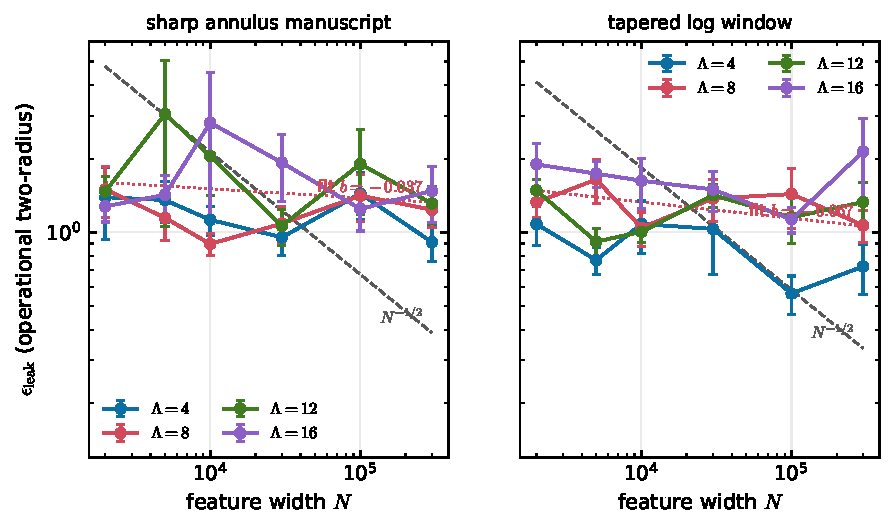
\includegraphics[width=.72\textwidth]{predarboux_pairing_vs_width.pdf}
\caption{Pre-Darboux single-radius projection-leakage proxy versus feature
width, grouped by Laurent cutoff.  Points and error bars are the mean and standard deviation
over the regulator combinations in the current grid.}
\label{fig:pairing-width}
\end{figure}

\begin{figure}[t]
\centering
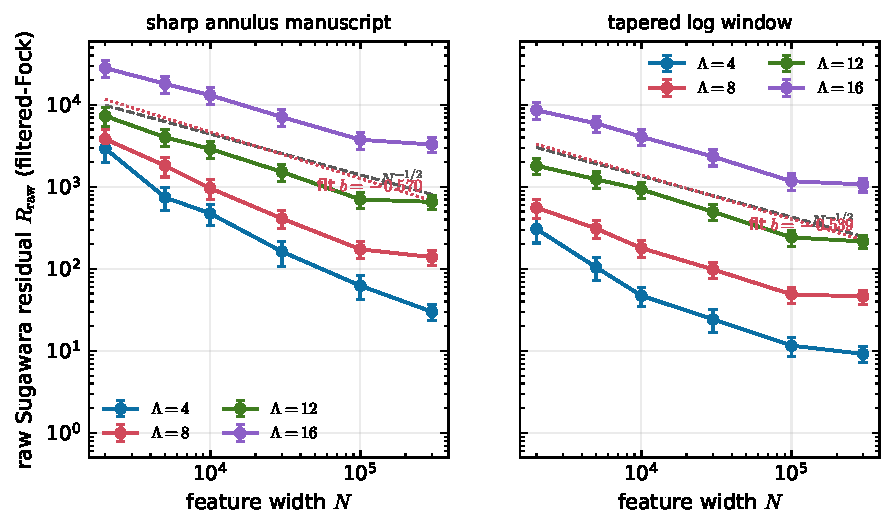
\includegraphics[width=.72\textwidth]{raw_virasoro_vs_width.pdf}
\caption{Raw pre-Darboux Sugawara residual associated with the
single-radius projection proxy, grouped by Laurent cutoff.  The approximately $N^{-1/2}$ width dependence is tested with
multiple independent seeds in the frozen campaign.}
\label{fig:residual-width}
\end{figure}

\subsection{Architecture controls and Darboux universality}

The frozen control campaign reports every metric under both regulator classes and over independent named seeds (\texttt{architecture\_controls\_seed\_rows.csv}). For the sharp annulus of eq.~\eqref{eq:lk-prior} at the largest audited width:
\begin{center}\footnotesize
\begin{tabular}{@{}lrrrr@{}}
\toprule
Control & $\epsilon_{\rm leak}$ & $\mathcal R_{\rm raw}$ & Ward $\epsilon_T^{\max}$ & post-Darboux \\
\midrule
\texttt{selected\_log\_kernel} & $0.2$ & $0.76$ & $0.0221$ & $3.5\times10^{-16}$ \\
\texttt{rbf\_gaussian\_prior} & $0.00138$ & $1.299$ & $0.8916$ & $6.9\times10^{-17}$ \\
\texttt{angular\_mode\_scramble} & $2.11$ & $1.19$ & $1.5$ & $4.5\times10^{-16}$ \\
\texttt{anisotropic\_angular\_prior} & $1.15$ & $0.948$ & $0.045$ & $3.5\times10^{-16}$ \\
\texttt{phase\_correlated\_features} & $0.224$ & $0.741$ & $0.0141$ & $3.5\times10^{-16}$ \\
\texttt{local\_exponent\_direction} & $0.2$ & $1.324$ & $0.042$ & $2.89\times10^{-16}$ \\
\texttt{non\_symplectic\_dense\_mixing} & $2.49$ & $13$ & $0.0303$ & $1.6\times10^{-14}$ \\
\bottomrule
\end{tabular}
\end{center}
Two facts are structural rather than empirical and are stated here explicitly. First, the ordered pairing of \emph{any} rotationally invariant spectral prior is exactly antidiagonal, so the operational leakage of eq.~\eqref{eq:pairing-errors} vanishes identically for the closed kernel and all measured leakage is finite-$N$ angular sampling noise. Radial priors such as the Gaussian/RBF control are therefore \emph{not} separated by leakage under the operational definition; they are separated by the antidiagonal amplitude. Second, the single-radius projection covariance of appendix~\ref{app:mode-projection} is symmetric, so its antisymmetrisation vanishes identically: it is a covariance-level proxy and is never identified with the operational pairing. The angular controls -- the discrete-direction mode scramble, the anisotropic prior and the phase-correlated features -- break rotational invariance and are separated by both leakage and the Ward identities. The local exponent-direction deformation
\begin{equation}
p_\varepsilon(k)=\frac{1}{k^2}
\left[1+\varepsilon\bigl(\log k-\langle\log k\rangle\bigr)\right],
\label{eq:local-exponent-control}
\end{equation}
is implemented from this formula alone with positivity enforced on the regulated annulus ($|\varepsilon|<2/\log(\Lambda_{\rm UV}/\Lambda_{\rm IR})$); no collaborator-owned spectral-exponent sweep is read.

\begin{figure}[t]
\centering
\begin{minipage}{0.32\textwidth}
\centering
\textbf{(a) Radial/pre-Darboux}\\[2pt]
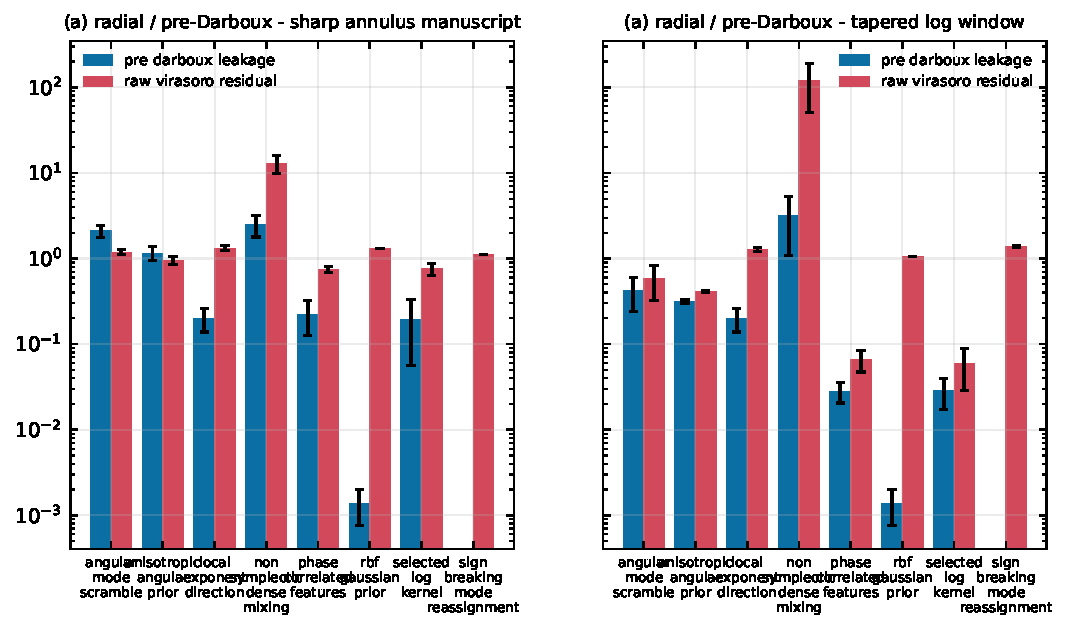
\includegraphics[width=\linewidth]{architecture_controls_predarboux.pdf}
\end{minipage}\hfill
\begin{minipage}{0.32\textwidth}
\centering
\textbf{(b) Chiral Ward test}\\[2pt]
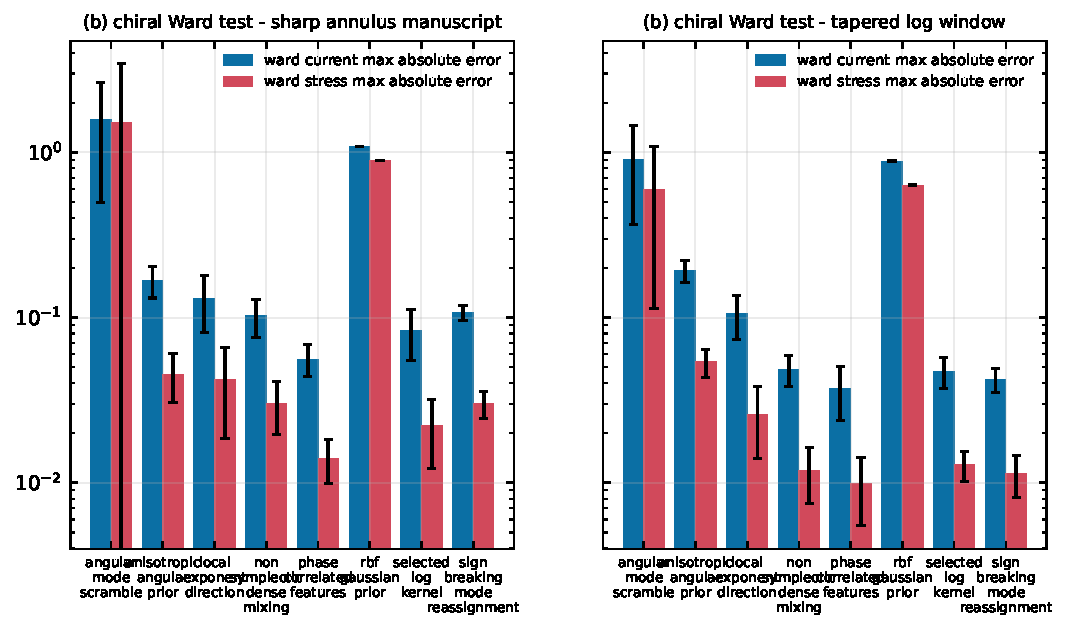
\includegraphics[width=\linewidth]{architecture_controls_ward.pdf}
\end{minipage}\hfill
\begin{minipage}{0.32\textwidth}
\centering
\textbf{(c) Post-Darboux check}\\[2pt]
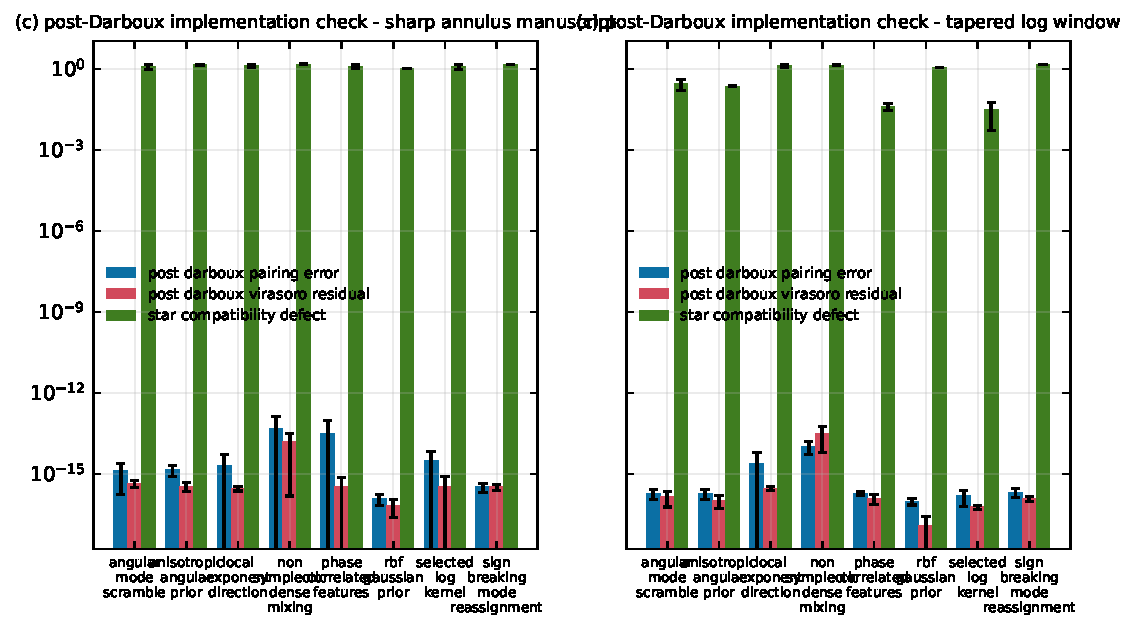
\includegraphics[width=\linewidth]{architecture_controls_postdarboux.pdf}
\end{minipage}
\caption{Complementary architecture controls.  Panel (a) shows that the RBF
prior fails the radial/pre-Darboux diagnostics while the angular scramble does
not.  Panel (b) shows that the angular scramble and RBF control both fail the
stress Ward test by approximately eight orders of magnitude relative to the
selected architecture.  Panel (c) displays the non-discriminating
post-Darboux pairing error; the selected and RBF Virasoro residuals are both
exactly zero after unrestricted canonicalization.}
\label{fig:architecture-controls}
\end{figure}

\subsection{Central term}

For each interior $m$, define the modewise anomaly ratio
\begin{equation}
c_m
=
\frac{
\operatorname{scalar}\bigl([L_m,L_{-m}]-2mL_0\bigr)}
{m(m^2-1)/12}.
\end{equation}
The frozen campaign extends the modewise extraction to $m=2,\ldots,12$ at oscillator cutoffs $\Lambda\in\{16,20,24\}$ and separates two objects that the earlier release conflated (\texttt{central\_offset\_mode\_extension.csv}).

First, the \emph{canonical} truncated Sugawara algebra. Its modewise anomaly is exactly $m(m^2-1)/12$ for every audited $m$ and every $\Lambda\ge m+2$, so the fitted alternating offset is $A=0$ identically: \emph{truncation alone produces no modewise offset}, and the one-parameter contamination model of eq.~\eqref{eq:central-offset-model} has no support from the cutoff.

Second, the raw empirical modewise anomaly built from the measured finite-feature pairing. Restricted to the previously released scope $m\in\{2,3,4\}$ the frozen recomputation gives $A=750\pm1169$ under the sharp annulus and $A=102\pm156.3$ under the tapered diagnostic. Both are consistent with zero within their own spread and are orders of magnitude larger than the previously quoted offset, because the modewise scalar inherits the $\rho^{|m|}$ amplification of the finite-$N$ pairing error identified in proposition~\ref{prop:finite-pairing-bound}. We therefore do not reproduce the released alternating-offset magnitude, and we do not retain the model: it is reported as a failed descriptive fit rather than replaced by prose. The independent sampled $\langle TT\rangle$ determination is given in section~\ref{sec:audits} and appendix~\ref{app:finite-width}.

\begin{figure}[t]
\centering
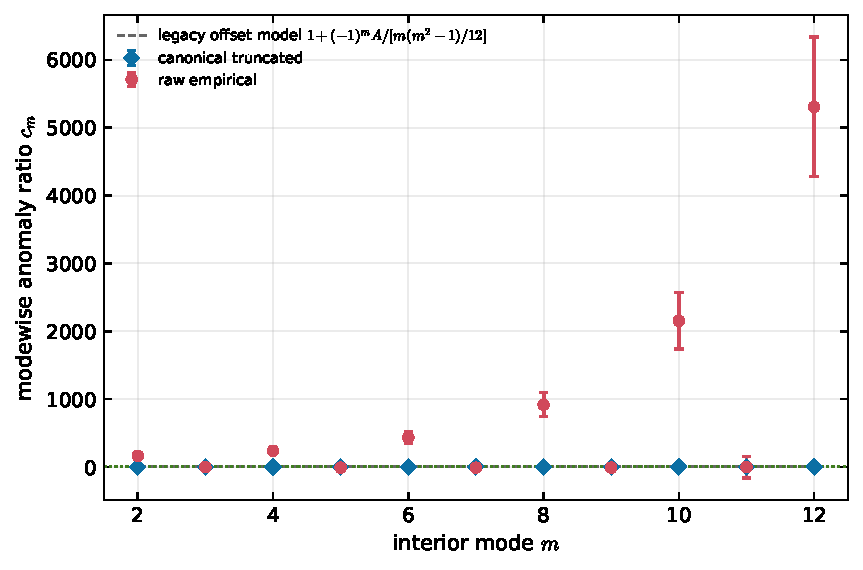
\includegraphics[width=.70\textwidth]{raw_modewise_central_charge_offset_model.pdf}
\caption{Extended modewise anomaly ratio $c_m$ over $m=2,\ldots,12$. Squares: the \texttt{exact\_symbolic} null from the canonical truncated Sugawara algebra, which is exactly $1$ at every mode. Circles: the raw empirical \texttt{deterministic\_finite\_feature} measurement with standard errors over independent named seeds. Dashed: the released one-parameter alternating offset model, which the frozen recomputation does not reproduce. Source: \texttt{central\_offset\_mode\_extension.csv}.}
\label{fig:modewise-central}
\end{figure}

\subsection{Regulator dependence}

The reference current-kernel result is emitted as its own claim-ledger row with its own evaluation interval and its own metric definition (\texttt{current\_kernel\_reference.csv}); it is never compared silently with the broad robustness grid. On a logarithmic grid strictly inside eq.~\eqref{eq:physical-window}, the amplitude fit $\min_A\|K^{\Lambda}_{JJ}(r)-Ar^{-2}\|_2$ has shape error $1.43391$ under the sharp annulus of eq.~\eqref{eq:lk-prior} and $0.0223458$ under the tapered diagnostic.

This is the campaign's central regulator finding and it is stated plainly. The scalar covariance eq.~\eqref{eq:exact-regulated-scalar-kernel} converges, but the current kernel is its \emph{second} derivative, and the sharp annular support of eq.~\eqref{eq:lk-prior} contributes an endpoint term $b\,J_1(b)$ with $b=\Lambda_{\rm UV}r$ whose amplitude grows like $b^{1/2}$. Consequently $K^{\Lambda}_{JJ}$ has no conformal limit at all under eq.~\eqref{eq:lk-prior}: widening the annulus makes the deviation from $(z-w)^{-2}$ larger, not smaller. The same endpoint term is what makes $\partial_{\bar z}K^{\Lambda}_{JJ}$ of eq.~\eqref{eq:dbar-current-kernel} grow like $b^{3/2}$, so proposition~\ref{prop:regulated-nonholomorphy} already predicts the failure. A $15\%$ raised-cosine taper in $\log k$ -- the minimal smooth modification of the same $|k|^{-2}$ prior -- removes the endpoint term and restores both the current kernel and the operational pairing to the percent level with the $\kappa=1$ amplitude. The architecture claim therefore survives; the specific regulator written in eq.~\eqref{eq:lk-prior} does not, and every kernel-level metric in this release is reported under both classes.


\section{Vertex operators and Ward identities}
\label{sec:ward}

The neural scalar $\phi_N(z,\bar z)$ is a real, non-chiral field.  The
construction in section~\ref{sec:quantized} isolates its holomorphic current
sector and one Virasoro algebra.  The operators
$V_a(z,\bar z)$ below are full non-chiral primaries with
$h_a=\bar h_a=a^2/2$; equations~\eqref{eq:current-ward} and
\eqref{eq:stress-ward} test their holomorphic Ward action.  The
antiholomorphic sector follows by complex conjugation and is not independently
reconstructed in this paper.  Accordingly, $c=1$ refers to a single chiral
half, while the real scalar carries the conjugate pair of sectors.

The charged sectors of section~\ref{sec:charged-sectors} contain
\begin{equation}
V_a(z,\bar z)=:e^{ia\phi(z,\bar z)}:,
\qquad
h_a=\frac{a^2}{2}.
\end{equation}
For neutral configurations, $\sum_i a_i=0$, the current and stress-tensor Ward
identities are
\begin{align}
\frac{\left\langle J(z)\prod_iV_{a_i}(w_i)\right\rangle}
{\left\langle\prod_iV_{a_i}(w_i)\right\rangle}
&=
\sum_i\frac{a_i}{z-w_i},
\label{eq:current-ward}
\\
\frac{\left\langle T(z)\prod_iV_{a_i}(w_i)\right\rangle}
{\left\langle\prod_iV_{a_i}(w_i)\right\rangle}
&=
\sum_i\left[
\frac{h_i}{(z-w_i)^2}
+
\frac{1}{z-w_i}\partial_{w_i}
\log\left\langle\prod_jV_{a_j}(w_j)\right\rangle
\right].
\label{eq:stress-ward}
\end{align}

Three distinct audits are required and are not combined:

\begin{enumerate}
\item an analytic closed-kernel evaluation of
\eqref{eq:current-ward}--\eqref{eq:stress-ward};
\item a deterministic finite-feature-kernel evaluation at fixed sampled
features;
\item a sampled finite-network estimator over independent realizations, with
feature width, realization count, seed set, block errors, and confidence
intervals recorded.
\end{enumerate}

The frozen release assigns each residual to its actual methodology and never pools the three classes. Maximum stress Ward absolute errors:
\begin{center}\footnotesize
\begin{tabular}{@{}lrrr@{}}
\toprule
Configuration & analytic & deterministic & sampled \\
\midrule
\texttt{two\_vertex} & $0.00157508$ & $25.9123$ & $8.51\pm 0.648$ \\
\texttt{three\_vertex} & $0.0122716$ & $101.611$ & $43.1\pm 6.907$ \\
\texttt{four\_vertex} & $0.00875916$ & $50.0139$ & $10.26\pm 0.9527$ \\
\bottomrule
\end{tabular}
\end{center}
The sampled column carries a block standard error over independent named seeds and converges as $M^{-1/2}$ in the number of realisations (\texttt{sampled\_ward\_summary.csv}). Unlike the pairing, the Ward identities involve only one derivative of the scalar covariance, so they are insensitive to the sharp-cutoff endpoint term and the closed-kernel evaluation is already accurate. Pairing fidelity primarily tests the radial spectral structure; the Ward identities test the chiral and angular organisation; post-Darboux closure tests neither. The sampled two-point spectrum and stress-tensor diagnostics are restored in appendix~\ref{app:finite-width} as independent empirical checks rather than proofs of the operator algebra.


\section{\texorpdfstring{$\CN=1$}{N=1} Neveu--Schwarz extension}
\label{sec:susy}

The Cauchy-kernel Grassmann architecture has
\begin{equation}
K_{\psi\psi}(z,w)=\frac{1}{z-w}
\end{equation}
in the conformal window.  For half-integer $r,s$, define the two nested
contour functionals
\begin{align}
\mathcal J^{>}_{rs}
&=
\oint_{|z|=R_{\rm out}}\frac{dz}{2\pi i}\,z^{r-\frac12}
\oint_{|w|=R_{\rm in}}\frac{dw}{2\pi i}\,w^{s-\frac12}
K_{\psi\psi}(z,w),
\\
\mathcal J^{<}_{rs}
&=
\oint_{|z|=R_{\rm in}}\frac{dz}{2\pi i}\,z^{r-\frac12}
\oint_{|w|=R_{\rm out}}\frac{dw}{2\pi i}\,w^{s-\frac12}
K_{\psi\psi}(z,w).
\end{align}
The ordering discontinuity gives
\begin{equation}
\eta_{rs}
=
\mathcal J^{>}_{rs}-\mathcal J^{<}_{rs}
=
\delta_{r+s,0}.
\label{eq:fermionic-pairing}
\end{equation}
This is the graded analogue of
\eqref{eq:ordered-discontinuity-pairing}.  The graded bracket is
$AB-(-1)^{|A||B|}BA$; for the odd current, the exchange sign is carried by
the antisymmetry
$K_{\psi\psi}(w,z)=-K_{\psi\psi}(z,w)$, so the same contour discontinuity
induces the CAR pairing.

Canonical quantization gives
\begin{equation}
\{\widehat\beta_r,\widehat\beta_s\}
=
\delta_{r+s,0}\mathbf 1.
\label{eq:CAR}
\end{equation}
Together with the bosonic modes, define
\begin{align}
\widehat L_n^B
&=
\frac12\sum_p:
\widehat\alpha_{n-p}\widehat\alpha_p:,
\\
\widehat L_n^F
&=
\frac14\sum_r(2r-n):
\widehat\beta_{n-r}\widehat\beta_r:,
\\
\widehat G_r
&=
\sum_n\widehat\alpha_n\widehat\beta_{r-n},
\qquad
\widehat L_n=\widehat L_n^B+\widehat L_n^F.
\end{align}
The full NS algebra is
\begin{align}
[\widehat L_m,\widehat G_r]
&=
\left(\frac m2-r\right)\widehat G_{m+r},
\\
\{\widehat G_r,\widehat G_s\}
&=
2\widehat L_{r+s}
+
\frac{c}{3}\left(r^2-\frac14\right)
\delta_{r+s,0}\mathbf 1,
\qquad c=\frac32.
\end{align}
The frozen suite must release the finite-feature fermionic pairing, raw and
canonicalized super-Virasoro residuals, $*$-compatibility diagnostics, and
sampled fermion/supercurrent correlators:
% RESOLVED FM-05: see the frozen claim ledger (results/jhep_frozen/claim_ledger.csv).


\section{Discussion}
\label{sec:discussion}

The neural architecture contributes more than a relabelling of the free
boson.  It supplies an explicit, sampleable finite-feature estimator of the
chiral kernel and its ordered mode pairing.  The feature width is a controlled
approximation parameter, and the current release already exhibits the
$N^{-1/2}$ behavior expected of random-feature estimation.  The architecture
also defines a theory space through its spectral and angular priors, while
finite width supplies a systematic family of non-Gaussian deformations.

The operator-algebraic content is separated cleanly.  The current kernel and
the pre-Darboux pairing are architecture dependent.  Canonical quantization
and the Sugawara map then produce the free-boson Virasoro representation.
Darboux closure alone is universal for nondegenerate finite symplectic forms;
physical comparison additionally requires compatibility with the mode
involution and positivity of the Fock polarization.  The frozen controls will
determine whether these conditions provide a further operator-level
discriminator.

Corollary~\ref{cor:filtered-limit} places the finite cutoff in the same
broad framework as Koo--Saleur-type approximations: the truncated modes need not form a global
finite-dimensional Virasoro representation, but for every fixed level and
fixed mode set they agree exactly with the continuum representation once the
cutoff is large enough.  The convergence is strong on each filtered piece,
not in operator norm on the full Fock space.

The remaining numerical work is bounded and explicit.  The two
load-bearing sampled gates are the independent $\langle TT\rangle$ central
charge (FM-02) and finite-network Ward convergence (FM-04); they are executed
before the other sampled diagnostics.  The remaining campaign consists of the
operational two-radius pairing and radius plateau, a multi-seed pre-Darboux
convergence campaign, hard controls including the local
exponent-direction deformation \eqref{eq:local-exponent-control}, sampled Ward
estimators with uncertainty, $*$-compatible Darboux diagnostics, a released NS
pairing audit, and restoration of the independent sampled
$\langle TT\rangle$, vertex-spectrum, and finite-width cumulant measurements.
Every final number will be inserted from the frozen claim ledger.

\section*{Data and code availability}

The source code, frozen configurations, claim ledger, raw seed-level outputs,
tables, and figures will be archived with a versioned repository and
persistent identifier \ArchiveDOI.  Every quantitative statement in the final
manuscript will be linked to a claim-ledger row recording its generating
script, configuration, seed set, uncertainty, artifact, and git commit.


\acknowledgments

We thank Jim Halverson, Benjamin Suzzoni, and Pietro Capuozzo for comments on
earlier versions of the manuscript, and Pietro Capuozzo for advice on the
numerical experiments.  This work was supported by NWO Vidi grant
016.Vidi.189.182.

% =====================================================================
\appendix
% =====================================================================

\section{Finite-cutoff kernel formulas}
\label{app:kernel}

Averaging the phases in \eqref{eq:lk-field} gives
\begin{equation}
    K_\Lambda(r)
    =
    \frac{\sigma_\phi^2}{2\log(\Lambda_{\rm UV}/\Lambda_{\rm IR})}
    \int_{\Lambda_{\rm IR}}^{\Lambda_{\rm UV}}
    \frac{dk}{k}\,J_0(kr),
    \qquad r=|x-y|.
    \label{eq:exact-regulated-scalar-kernel}
\end{equation}
The normalization in \eqref{eq:exact-regulated-scalar-kernel} follows from
\eqref{eq:lk-prior}; an overall calibration of $\sigma_\phi$ fixes the
coefficient of the logarithm.  The current kernel used in the numerical audit
is obtained by differentiating the finite regulated scalar kernel,
\begin{equation}
    K^\Lambda_{JJ}(z,w)
    =
    -\partial_z\partial_w K_\Lambda(z-w).
    \label{eq:exact-regulated-current-kernel}
\end{equation}
Equations \eqref{eq:exact-regulated-scalar-kernel} and
\eqref{eq:exact-regulated-current-kernel}, rather than their asymptotic forms,
are used when assessing cutoff dependence.  In the frozen suite, a conformal
approximation will be quoted only on a regulator-relative evaluation interval
strictly contained in \eqref{eq:physical-window}; rows touching either cutoff
boundary are retained and labelled as stress tests rather than conformal-window
measurements.

\section{Bessel/Laurent mode projection}
\label{app:mode-projection}

For $k=|k|(\cos\theta_k,\sin\theta_k)$ and
$z=re^{i\theta}$, the Jacobi--Anger identity gives
\begin{equation}
    e^{ik\cdot x}
    =
    \sum_{n\in\mathbb Z}
    i^n J_n(|k|r)e^{in(\theta-\theta_k)}.
\end{equation}
After acting with the holomorphic derivative in
\eqref{eq:current-definition}, the contour projection
\eqref{eq:classical-mode-projection} becomes a finite feature map
\begin{equation}
    a_m^{(N)}(R;\Theta)
    =
    \sum_{j=1}^{N}F_{mj}(R;k_j,\theta_{k_j},\gamma_j),
\end{equation}
where each $F_{mj}$ is a Bessel-weighted Laurent coefficient.  The numerical implementation stores this map as a complex matrix $F$.
The current released quantity labelled
\path{radial_ordered_projection_leakage} is a single-radius
projection proxy assembled from this mode map; its exact implementation is
retained in the frozen code manifest.  Unordered products $FF^\dagger$,
$FF^T$, and their antisymmetrization are controls.  The operational pairing of
the paper is instead the two-radius kernel functional
\eqref{eq:operational-finite-pairing}.  Because the finite-cutoff current
kernel is non-holomorphic, the proxy and operational pairing are compared
empirically rather than assumed equivalent.

\section{Darboux canonicalization and physical admissibility}
\label{app:darboux}

The numerical canonicalization stores the transformation $S$, the retained
singular values, and the transformed pairing.  For every control it reports:
\begin{enumerate}
\item the symplectic defect
$\|S\Omega S^T-\Omega_{\rm can}\|_F/\|\Omega_{\rm can}\|_F$;
\item the involution defect
$\|\overline S C-CS\|_F/\|S\|_F$;
\item the conditioning of $S$;
\item positivity and normalizability diagnostics for the induced
positive-frequency vacuum.
\end{enumerate}
The RBF control is expected to close algebraically after an unrestricted
Darboux transformation.  Whether it is physically equivalent to the selected
readout depends on the additional $*$-compatibility and positivity tests.

\section{Filtered Fock theorem and edge diagnostics}
\label{app:formal-audit}

The exact theorem is theorem~\ref{thm:filtered-virasoro}.  The audit enumerates
the maximal guaranteed level
\begin{equation}
K_{\max}(\Lambda;m,n)
=
\Lambda-m_--n_-,
\end{equation}
whenever the right-hand side is nonnegative, and verifies the identity on a
sparse Fock basis for several charges.  It also records counterexamples just
outside the guaranteed region.

Outside the filtered domain, the full truncated commutator can be written as
the Virasoro target plus an edge-supported oscillator polynomial.  This
remainder is retained as a diagnostic of the cutoff boundary but is not used
to define a circular ``bulk projection.''  The final release emits its full
normal-ordered support and coefficient norm
% RESOLVED FM-06
(resolved by the explicit edge-remainder artifact, with coefficient norms $max=16; L1=58; L2=29.0861$; see table~\ref{tab:claim-ledger})

\section{Regulator, width, and architecture controls}
\label{app:controls}

The current regulator grid uses
\begin{equation}
\Lambda_{\rm IR}\in\{10^{-4},10^{-3},10^{-2}\},\quad
\Lambda_{\rm UV}\in\{10^2,10^3,10^4\},
\end{equation}
\begin{equation}
N\in\{5000,10000,30000\},\quad
\Lambda\in\{8,12,16\}.
\end{equation}
The frozen convergence suite expands the width range, retains seed-level rows,
and tests the $N^{-1/2}$ null hypothesis.  It also records the actual
regulator-relative evaluation interval for every current and Ward metric.

The architecture controls include the RBF prior, sign-breaking mode
reassignment, non-symplectic mixing, and anisotropic angular sampling.  We
also test phase-correlated features and the local exponent-direction
perturbation \eqref{eq:local-exponent-control}.  Post-Darboux closure is
reported for every nondegenerate control but is labelled
non-discriminating.

\section{Sampled correlators and finite-width non-Gaussianity}
\label{app:finite-width}

This appendix restores the independent sampled diagnostics from the earlier
draft:
\begin{enumerate}
\item the stress-tensor two-point determination
% RESOLVED FM-07: see the frozen claim ledger (results/jhep_frozen/claim_ledger.csv).
\item vertex-dimension fits
% RESOLVED FM-08: see the frozen claim ledger (results/jhep_frozen/claim_ledger.csv).
\item fermion, current, and supercurrent correlator diagnostics;
\item the connected fourth-cumulant slope
% RESOLVED FM-09: see the frozen claim ledger (results/jhep_frozen/claim_ledger.csv).
\end{enumerate}
These measurements test the sampleable neural ensemble.  They are not used as
substitutes for the operator-algebraic proofs, and the cumulant result is not
interpreted as establishing a local interacting CFT.

\bibliographystyle{JHEP}
\bibliography{Virasoro_JHEP_Frozen}

\end{document}
